\documentclass[a4paper,oneside,10pt]{book}
\usepackage[english]{babel}
\usepackage[portrait,a4paper,margin=2.0cm,headsep=5mm]{geometry}
\usepackage[utf8]{inputenc}
\usepackage[T1]{fontenc}
\usepackage{lmodern}
\usepackage{longtable}
\usepackage[usenames,dvipsnames]{xcolor}
\usepackage[colorlinks=true, linkcolor=blue, urlcolor=blue]{hyperref}
\hypersetup{hidelinks}
\usepackage{array}
\usepackage{graphicx}
\usepackage[labelfont=bf,singlelinecheck=false,format=plain,,justification=justified,indention=0cm]{caption}
\usepackage{listings}
\usepackage{mdframed}

% see ftp://ftp.tex.ac.uk/tex-archive/macros/latex/contrib/listings/listings.pdf

\definecolor{background}{RGB}{255,255,255}
\definecolor{hellgelb}{rgb}{1,1,0.8}
\definecolor{colKeys}{RGB}{127,0,85}
\definecolor{colIdentifier}{rgb}{0,0,0}
\definecolor{colComments}{RGB}{63,127,95}
\definecolor{colString}{RGB}{42,0,255}

% for all listings
\lstset{%
    float=hbp,%
    basicstyle=\ttfamily\small, %
    identifierstyle=\color{colIdentifier}, %
    keywordstyle=\color{colKeys}\bf, %
    stringstyle=\color{colString}, %
    commentstyle=\color{colComments}, %
    columns=flexible, %
    tabsize=2, %
    frame=none, %
    extendedchars=true, %
    showspaces=false, %
    showstringspaces=false, %
    numbers=left, %
    numberstyle=\tiny, %
    breaklines=true, %
    backgroundcolor=\color{background}, %
    breakautoindent=true, %
    captionpos=b%
}

\lstdefinelanguage{ROOM}
{morekeywords={
	handle,
	usercode,
	external,
	outgoing,
	ChoicePoint,
	of,
	semantics,
	initial,
	Attribute,
	import,
	SPP,
	Binding,
	ExitPoint,
	or,
	exit,
	Port,
	ptReal,
	usercode3,
	incoming,
	usercode2,
	usercode1,
	ExternalType,
	SubSystemRef,
	cond,
	conjugated,
	private,
	PrimitiveType,
	SAP,
	PortClass,
	SubSystemClass,
	DataClass,
	sync,
	ActorClass,
	guard,
	ptCharacter,
	ptInteger,
	do,
	LayerConnection,
	TransitionPoint,
	Message,
	relay_sap,
	void,
	LogicalSystem,
	my,
	CompoundProtocolClass,
	ref,
	Behavior,
	ActorInstanceMapping,
	Structure,
	triggers,
	EntryPoint,
	Operation,
	SubProtocol,
	action,
	RefinedState,
	extends,
	conjugate,
	and,
	Interface,
	default,
	cp,
	StateMachine,
	satisfied_by,
	Transition,
	ptBoolean,
	sub,
	model,
	from,
	sends,
	RoomModel,
	ActorRef,
	RefinedTransition,
	LogicalThread,
	ServiceImplementation,
	ProtocolClass,
	abstract,
	regular,
	in,
	async,
	subgraph,
	State,
	entry,
	datadriven,
	eventdriven,
	out,
	handler,
	AnnotationType,
	optional,
	mandatory,
	attribute,
	ActorBehavior,
	target,
	Enumeration,
}
sensitive=false,
morecomment=[l]{//},
morecomment=[s]{/*}{*/},
morestring=[b]",
} 


\lstdefinelanguage{Config}
{morekeywords={
	polling,
	timer,
	ms,
	model,
	Attr,
	file,
	path,
	from,
	InterfaceItem,
	ActorClassConfig,
	write,
	false,
	read,
	import,
	min,
	max,
	ProtocolClassConfig,
	regular,
	true,
	ActorInstanceConfig,
	conjugate,
	dynamic,
	configuration,
	Port,
	SubSystemConfig,
	ConfigModel,
	user,
	import,
	user,
	constructor,
}
sensitive=false,
morecomment=[l]{//},
morecomment=[s]{/*}{*/},
morestring=[b]",
} 

\lstdefinelanguage{etPhys}
{morekeywords={
	ns,
	NodeRef,
	model,
	interval,
	RuntimeClass,
	singleThreaded,
	runtime,
	from,
	multiThreaded,
	DefaultThread,
	msgpoolsize,
	execmode,
	mixed,
	blocked,
	import,
	msgblocksize,
	Thread,
	priomin,
	polled,
	PhysicalSystem,
	ms,
	PhysicalModel,
	us,
	stacksize,
	NodeClass,
	priomax,
	prio,
}
sensitive=false,
morecomment=[l]{//},
morecomment=[s]{/*}{*/},
morestring=[b]",
} 

\lstdefinelanguage{etMap}
{morekeywords={
	model,
	MappingModel,
	SubSystemMapping,
	import,
	from,
	Mapping,
	ThreadMapping,
}
sensitive=false,
morecomment=[l]{//},
morecomment=[s]{/*}{*/},
morestring=[b]",
} 

\lstdefinelanguage{PlainText}
{morekeywords={
}
sensitive=false,
morecomment=[l]{//},
morecomment=[s]{/*}{*/},
morestring=[b]",
} 


\setlength{\parindent}{0pt}  
\setlength{\parskip}{4pt plus 1pt minus 0pt}  % Abstand zwischen Absaetzen
 \nonfrenchspacing
 \sloppy

\newcommand{\specialcell}[2][c]{%
  \begin{tabular}[#1]{@{}c@{}}#2\end{tabular}}

% the robust command prevents premature macro expansion
% but the entry in the PDF structure is wrong (redblueTrice)
%\DeclareRobustCommand{\eTrice}{{\color{blue}e}{\color{red}Trice}{}}

% defining these colors fixes a problem with the plain newcommand
% but still the PDF structure entries are wrong (reblueTrice)
\definecolor{RED}{RGB}{255,0,0}
\definecolor{BLUE}{RGB}{0,0,255}
\newcommand{\eTrice}{{\color{blue}e}{\color{red}Trice}{}}

% the following command makes eTrice vanish completely from the PDF structure
%\usepackage{etoolbox}
%\newrobustcmd{\eTrice}{{\color{blue}e}{\color{red}Trice}{}}

\newcommand{\myparagraph}[1]{\paragraph{#1}\mbox{}\\}
%\newcommand{\room}[1]{\textcolor{RedViolet}{\texttt{#1}}}
\newcommand{\room}[1]{\textcolor{Fuchsia}{\textbf{#1}}}
\renewcommand{\familydefault}{\sfdefault}
 

\begin{document}

\begin{titlepage}

\begin{center}


\includegraphics[width=0.4\textwidth]{images/logo/eTRICE-logo.png}

\Huge \eTrice{} Documentation

\Large version 0.5.0

\large \eTrice{} committers and contributors

\vfill

% Bottom of the page
{\large \today}

\end{center}

\end{titlepage}

\tableofcontents

\chapter{Introduction}

\section{\eTrice{} Overview}

\subsection{What is \eTrice{}?}

\eTrice{} provides an implementation of the ROOM modeling language (Real Time Object Oriented Modeling) 
together with editors, code generators for Java, C++ and C code and exemplary target middleware.

The model is defined in textual form (Xtext) with graphical editors (Graphiti) for the structural and 
behavioral (i.e. state machine) parts.

\subsection{Reduction of Complexity}

\eTrice{} is all about the reduction of complexity:

\begin{itemize}
\item structural complexity
	\begin{itemize}
	\item by explicit modeling of hierarchical Actor containment, layering and inheritance
	\end{itemize}
\item behavioral complexity
	\begin{itemize}
	\item by hierarchical state machines with inheritance
	\end{itemize}
\item team work complexity
	\begin{itemize}
	\item because loosely coupled Actors provide a natural way to structure team work
	\item since textual model notation allows simple branching and merging
	\end{itemize}
\item complexity of concurrent \& distributed systems
	\begin{itemize}
	\item because loosely coupled Actors are deployable to threads, processes, nodes
	\end{itemize}
\item complexity of variant handling and reuse (e.g. for product lines)
	\begin{itemize}
	\item by composition of existing Actors to new structures
	\item since Protocols and Ports make Actors replaceable
	\item by inheritance for structure, behavior and Protocols
	\item by making use of model level libraries 
	\end{itemize}
\item complexity of debugging
	\begin{itemize}
	\item model level debugging: state machine animation, data inspection and manipulation, message injection, 
	generated message sequence charts
	\item model checking easier for model than for code (detect errors before they occur)
	\end{itemize}
\end{itemize}

\section{Introduction to the ROOM Language}

\subsection{Scope of ROOM}

This chapter will give a rough overview of what ROOM (\textbf{R}eal-time
\textbf{O}bject-\textbf{O}riented \textbf{M}odeling) is and what it is good for.
It will try to answer the following questions:

\begin{itemize}
\item Where does it come from?
\item Which kind of SW-Systems will be addressed?
\item What is the relation between object oriented programming and ROOM?
\item What are the benefits of ROOM?
\item Which consequences must be taken into account?
\end{itemize}

\subsubsection{Where does it come from?}

ROOM was developed in the 1990th on the background of the upcoming mobile applications with the goal to
manage the complexity of such huge SW-Systems. From the very beginning ROOM has focused on a certain type
of SW-Systems and is, in contrast to the UML, well suited for this kind of systems. In this sense, ROOM is
a DSL (Domain Specific Language) for distributed, event driven, real time systems. 

Bran Selic, Garth Gullekson and Paul T. Ward have published the concepts 1994 in the book
\textbf{Real-Time Object-Oriented Modeling}. The company \textit{ObjecTime}\texttrademark{}
developed a ROOM tool which was taken over by \textit{Rational SW}\texttrademark{} and later
on by \textit{IBM}\texttrademark.
The company \textit{Protos Software GmbH}\texttrademark{} also developed a ROOM tool called
\textit{Trice}\texttrademark{} for control software for production machines and automotive systems.
\textit{Trice}\texttrademark{} is the predecessor of \eTrice{} (see Introduction to \eTrice{}). 
 
From our point of view ROOM provides still the clearest, simplest, most complete and best suited modeling
concepts for the real time domain. All later proposals like the UML do not fit as well to this kind of problems.
 

\subsubsection{Which kind of SW-Systems will be addressed?}

As mentioned before ROOM addresses distributed, event driven, real time systems.
But what is a \emph{real time system}? ROOM defines a set of properties
which are typical for a real time system. These properties are:

\begin{itemize}
\item Timeliness
\item Dynamic internal structure
\item Reactiveness
\item Concurrency
\item Distribution
\item Reliability
\end{itemize}

Each of these properties has potential to make SW development complex. If a given system can be characterized
with a combination of or all of these properties, ROOM might be applied to such a system.  

As an example take a look at a washing machine. The system has to react to user interactions, has to handle
some error conditions like a closed water tap or a defective lye pump. It has to react simultaneously to all these inputs.
It has to close the water valve within a certain time to avoid flooding the basement. 
So, the system can be characterized as timely, concurrent and reactive. As long as the washing machine does
not transform to a laundry drier by itself, the system has no dynamic internal structure and as long as all functions
are running on a single micro controller the (SW)-system is not distributed. 
ROOM fits perfect to such a system.

A SW system which mainly consists of data transformations like signal/image processing or a loop controller
(e.g. a PID controller) cannot be characterized with any of the above mentioned properties. However, in the real
world most of the SW systems will be a combination of both. ROOM can be combined with such systems, so that for
example an actor provides a \emph{run to completion} context for calculating an image processing algorithm or a
PID controller.  

\subsubsection{What is the relation between OOP and ROOM?}

The relation between classical object oriented programming and ROOM is comparable to the relation between assembler
programming and C programming. It provides a shift of the object paradigm. The classical object
paradigm provides some kind of information hiding. Attributes can be accessed via access methods. Logical higher level
methods provide the requested behavior to the user.

But as the figure illustrates, the classical object paradigm does not care about concurrency issues. The threads of
control will be provided by the underlying operating system and the user is responsible to avoid access violations
by using those operating system mechanisms directly (semaphore, mutex).

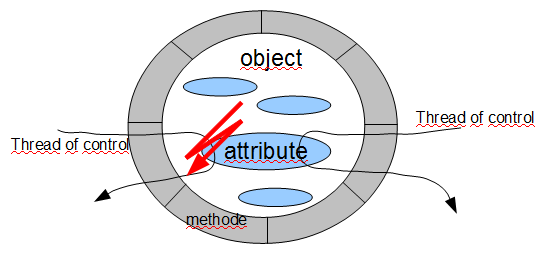
\includegraphics[width=0.6\textwidth]{images/010-RoomIntroduction02.png}

ROOM provides the concept of a logical machine (called actor) with its own thread of control. It provides some kind
of cooperative communication infrastructure with \emph{run to completion} semantics.
That makes developing of business logic easy and safe (see \ref{sec:basic_concepts} \nameref{sec:basic_concepts}). The logical machine provides an 
encapsulation shell including concurrency issues (see \ref{sec:run_to_completion} \nameref{sec:run_to_completion}). 

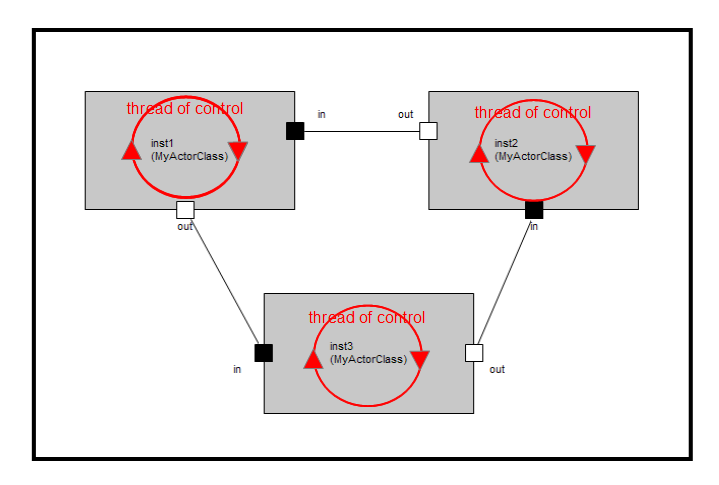
\includegraphics[width=0.8\textwidth]{images/010-RoomIntroduction03.png}

This thinking of an object is much more general than the classic one.  

\subsubsection{What are the benefits of ROOM?}

ROOM has a lot of benefits and it depends on the users point of view which is the most important one. From a general
point of view the most important benefit is, that ROOM allows to create SW systems very efficient, robust and safe
due to the fact that it provides some abstract, high level modeling concepts combined with code generation and a
small efficient runtime environment.  

In detail:
\begin{itemize}
\item ROOM models contain well defined interfaces (protocols), which makes it easy to re-use components in different
applications or e.g. in a test harness. 
\item Graphical modeling makes it easy to understand, maintain and share code with other developers
\item Higher abstraction in combination with automated code generation provides very efficient mechanisms to
the developer. 
\item ROOM provides graphical model execution, which makes it easy to understand the application or find defects in
a very early phase. 
\end{itemize}

\subsubsection{Which consequences must be taken into account?}

Generating code from models will introduce some overhead in terms of memory footprint as well as performance.
For most systems the overhead will be negligible. However, the decision for using ROOM should be made explicitly
and it is always a trade off between development costs, time to market and costs in terms of a little bit more of
memory and performance. Thanks to the powerful component model, ROOM is especially well suited for the development
of software product lines with their need for reusable core assets.  
  
Care must be taken during the introduction of the new methodology. Due to the fact that ROOM provides a shift of the
object paradigm, developers and teams need a phase of adaption. Every benefit comes at a price.

\subsection{Basic Concepts}
\label{sec:basic_concepts}

\subsubsection{Actor, Port, Protocol}

The basic elements of ROOM are the actors with their ports and protocols.
The protocol provides a formal interface description. The port is an interaction
point where the actor interacts with its outside world. Each port has exactly one protocol
attached. The sum of all ports builds up the complete interface of an actor.
Each port can receive messages, with or without data, which are defined in the attached protocol.
Each message will be handled by the actor's behavior (state machine) or will be delegated to the actor's internal structure.

\begin{table}
\caption{Actor and Protocol Class Example}
\begin{tabular}{|l|l|}
\hline
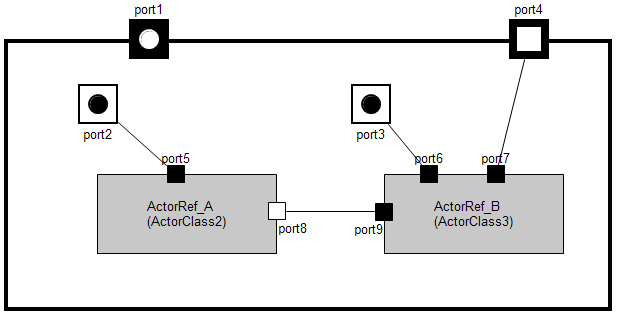
\includegraphics[scale=0.85]{images/040-ActorClass.png} & 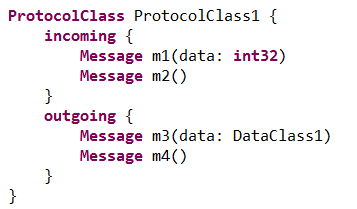
\includegraphics[scale=0.85]{images/040-ProtocolClassTextualNotation.png} \\ \hline
\textbf{Actor with sub actors} & \textbf{Protocol definition} \\ \hline
\end{tabular}
\end{table}

The actor provides access protection for its own attributes (including complex types, i.e. classical objects), 
including concurrency protection. An actor has neither public attributes nor public operations. The only 
interaction with the outside world takes place via interface ports. This ensures a high degree of 
re-usability on the actor level and provides an effective and safe programming model to the developer. 

Receiving a message via a port will trigger the internal state machine. A transition will be executed 
depending on the message and the current state. Within this transition, detail level code will be executed 
and response messages can be sent.

With this model, a complex behavior can be divided into many relatively simple, linked actors. To put it the 
other way round: The complex behavior will be provided by a network of relatively simple components which 
are communicating with each other via well defined interfaces.


\subsubsection{Hierarchy in Structure and Behavior}

ROOM provides two types of hierarchy. Behavioral hierarchy and structural hierarchy. Structural hierarchy 
means that actors can be nested to arbitrary depth. Usually you will add more and more details to your 
application with each nesting level. That means you can focus yourself on any level of abstraction with 
always the same element, the actor. Structural hierarchy provides a powerful mechanism to divide your 
problem in smaller pieces, so that you can focus on the level of abstraction you want to work on. 

The actor's behavior will be described with a state machine. A state in turn may contain sub states. This 
is another possibility to focus on an abstraction level. Take the simple FSM from the blinky actor from 
the blinky tutorial. 
   
Top level:

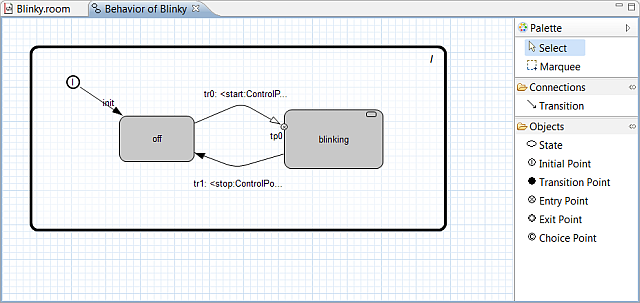
\includegraphics[width=0.8\textwidth]{images/020-Blinky15.png}

\textit{blinking} Sub machine:

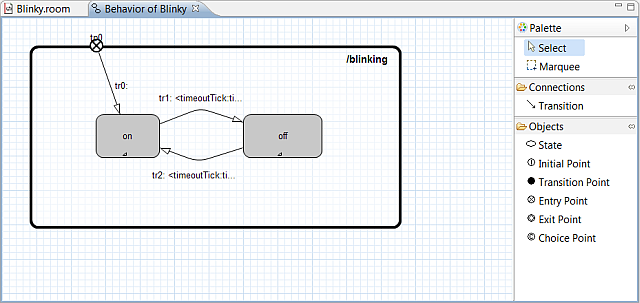
\includegraphics[width=0.8\textwidth]{images/020-Blinky151.png}

From an abstract point of view there is a state \textit{blinking}. But a simple LED is not able to blink 
autonomously. Therefore you have to add more details to your model to make a LED blinking, but for the 
current work it is not of interest how the blinking is realized. This will be done in the next lower level 
of the hierarchy. 

This simple example might give an idea how powerful this mechanisms is.

The hierarchical FSM provides a rich tool box to describe real world problems (see chapter \ref{sec:room_concepts} \nameref{sec:room_concepts}).

\subsubsection{Layering}

Layering is another well known form of abstraction to reduce complexity in the structure of systems. ROOM 
is probably the only language that supports layering directly as a language feature.
Layering can be expressed in ROOM by actors with specialized ports, called \emph{Service Access Points} 
(SAP) and \emph{Service Provision Points} (SPP).

The actor that provides a service implements an SPP and the client of that service implements an SAP. The 
layer connection connects all SAPs of a specific protocol within an actor hierarchy with an SPP that 
implements the service. From the actor's point of view, SAPs and SPPs behave almost like ports.

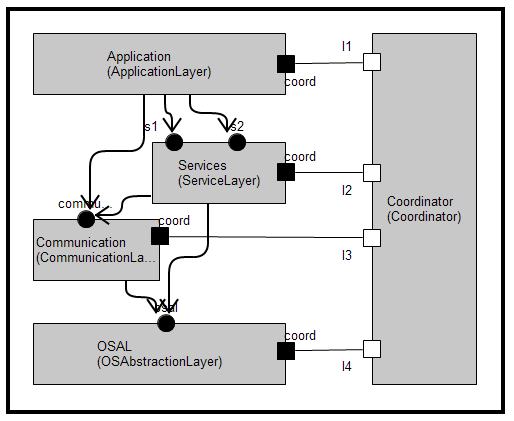
\includegraphics{images/010-LayerExample.png}

The example shows a layered model. The layer connections define e.g. that the \textit{ApplicationLayer} 
can only use the services of the \textit{ServiceLayer} and the \textit{CommunicationLayer}. Actors inside 
the \textit{ApplicationLayer} that implement an SAP for those services are connected directly to the 
implementation of the services. 
Layering and actor hierarchies with port to port connections can be mixed on every level of granularity. 

\subsubsection{Run to Completion}
\label{sec:run_to_completion}

\emph{Run to completion} (RTC) is a very central concept of ROOM. It enables the developer to 
concentrate on the functional aspects of the system. The developer doesn't have to care about concurrency 
issues all the time. This job is concentrated to the system designer in a very flexible way.
What does \emph{run to completion} mean:
RTC means that an actor, which is processing a message, can not receive the next message as long as the 
processing of the current message has been finished. Receiving of the next message will be queued by the 
underlying run time system.

Note: It is very important not to confuse \emph{run to completion} and \emph{cooperative multi threading}.
Run to completion means that 
an actor will finish the processing of a message before he can receive a new one (regardless of its 
priority). That does \emph{not} mean that an actor cannot be preempted from an higher priority thread of control. 
But even a message from this higher prior thread of control will be queued until the current processing 
has been finished. 

With this mechanism all actor internal attributes and data structures are protected. Due to the fact that 
multiple actors share one thread of control, all objects are protected which are accessed from one thread 
of control but multiple actors. This provides the possibility to decompose complex functionality into 
several actors without the risk to produce access violations or dead locks.

\subsection{Execution Models}

Since from ROOM models executable code can be generated, it is important to define the way the actors are 
executed and communicate with each other. The combination of communication and execution is called the 
\emph{execution model}.
Currently the \eTrice{} tooling supports the \textbf{message driven}, the \textbf{data 
driven} and a mixture of both execution models. In future releases maybe also a synchronous
execution model will be supported, depending on the 
requirements of the community.

\subsubsection{Communication Methods}

\begin{itemize}
\item \textbf{message driven} -- asynchronous, non blocking, no return value:\\
Usually the message driven 
communication is implemented with message queues. Message queues are inherently asynchronous and enable a 
very good decoupling of the communicating parties.
\item \textbf{data driven} -- asynchronous, non blocking, no return value:\\
In data driven communication 
sender and receiver often have a shared block of data. The sender writes the data and the receiver polls 
the data.
\item \textbf{function call} -- synchronous, blocking, return value:\\
Regular function call as known in most 
programming languages.
\end{itemize}

\eTrice{} currently supports the two former communication methods.

\subsubsection{Execution Methods}

\begin{itemize}
\item \textbf{execution by receive event}: The message queue or the event dispatcher calls a 
\textbf{receive event} function of the message receiver and thereby executes the processing of the event.
\item \textbf{polled execution}: The objects are processed by a cyclic \textbf{execute} call
\item \textbf{execution by function call}: The caller executes the called object via function call
\end{itemize}

\eTrice{} currently supports the two former execution methods.

\subsubsection{Execution Models}

In present-day's embedded systems in most cases one or several of the following execution models are used:

\myparagraph{message driven}

The message driven execution model is a combination of message driven communication and execution by 
receive event.
This model allows for distributed systems with a very high throughput.
It can be deterministic but the determinism is hard to proof.
This execution model is often found in telecommunication systems and high performance automation control 
systems.

\myparagraph{data driven}

The data driven execution model is a combination of data driven communication and polled execution.
This model is highly deterministic and very robust, but the polling creates a huge performance overhead.
The determinism is easy to proof (simple mathematics). 
The execution model is also compatible with the execution model of control software generated by Tools 
like Matlab(TM) and LabView(TM).
This model is usually used for systems with requirements for safety, such as automotive and avionic systems.

\myparagraph{synchronous}

The synchronous execution model could also be called \emph{function calls}. 
This model in general is not very well suited to support the \emph{run to completion} semantics typical 
for ROOM models, but could also be generated from ROOM models. 
With this execution model also lower levels of a software system, such as device drivers, could be 
generated from ROOM models.


\chapter{Tutorials}

\chapter{Working with the eTrice Tutorials}

The eTrice Tutorials will help you to learn and understand the eTrice tool and concepts. ETrice supports 
several target languages. The concepts will not be explained for each language. 

Most of the common concepts will be described for Java as target language. To start with a new language the 
first steps to setup the workspace and to generate and run the first model will be described also. Target 
language specific aspects will be described as well.

Therefore the best way to start with eTrice is to follow the Java Tutorials and after that switch to your 
target language.  

\section{Setting up the Workspace for Java Projects}

After installation of eclipse and the \eTrice{} plug in, your workspace should look like this:  

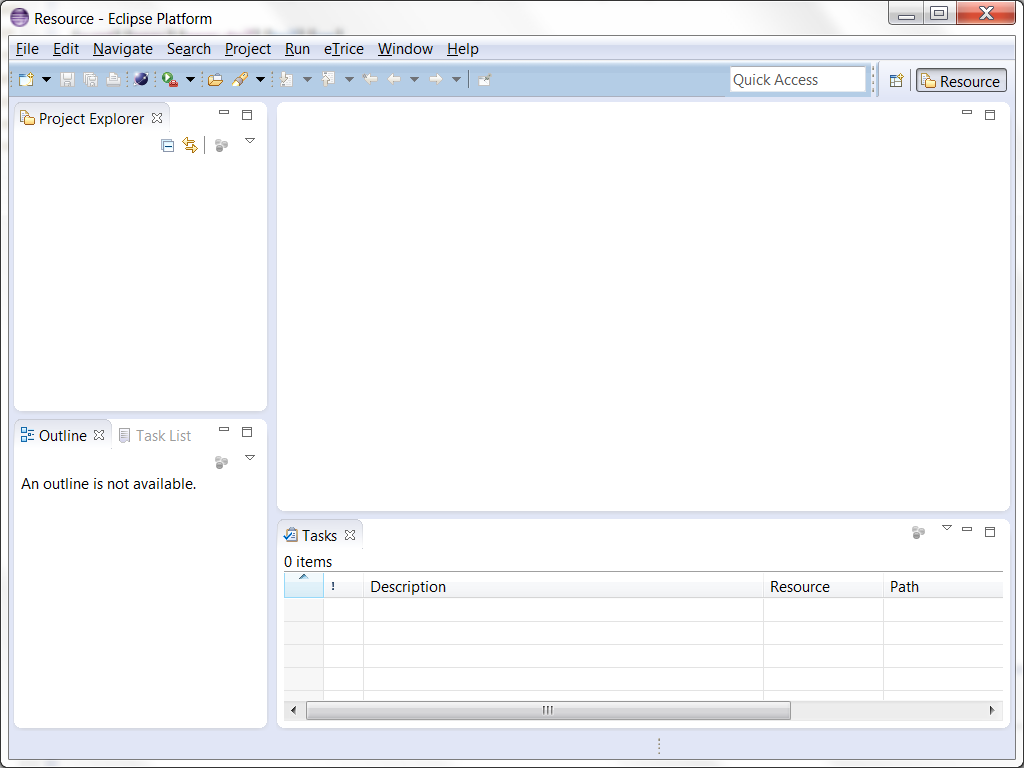
\includegraphics[width=0.8\textwidth]{images/013-SetupWorkspace01.png}
% !images/013-SetupWorkspace01.png!

Just the \textit{\eTrice{}} menu item is visible of the installed \eTrice{} plugins.

Select the menu \textbf{File->New->Other}

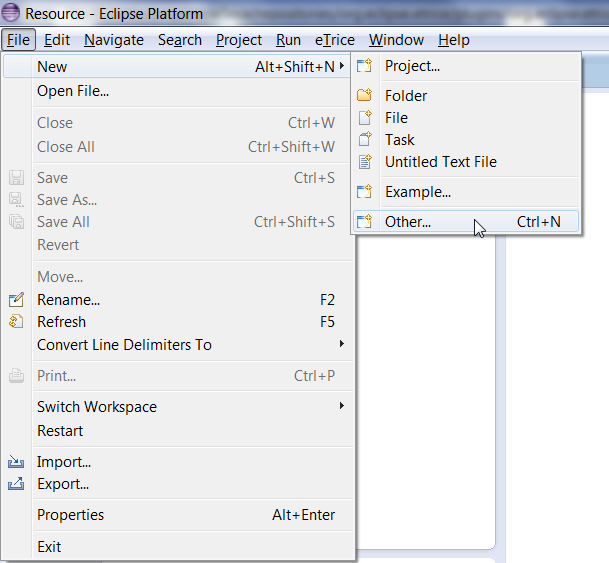
\includegraphics[width=0.8\textwidth]{images/013-SetupWorkspace02.png}
% !images/013-SetupWorkspace02.png!

Open the \textit{\eTrice{}} tab and select \textit{\eTrice{} Java Runtime}

Press \textit{Next} and \textit{Finish} to install the Runtime into your workspace.

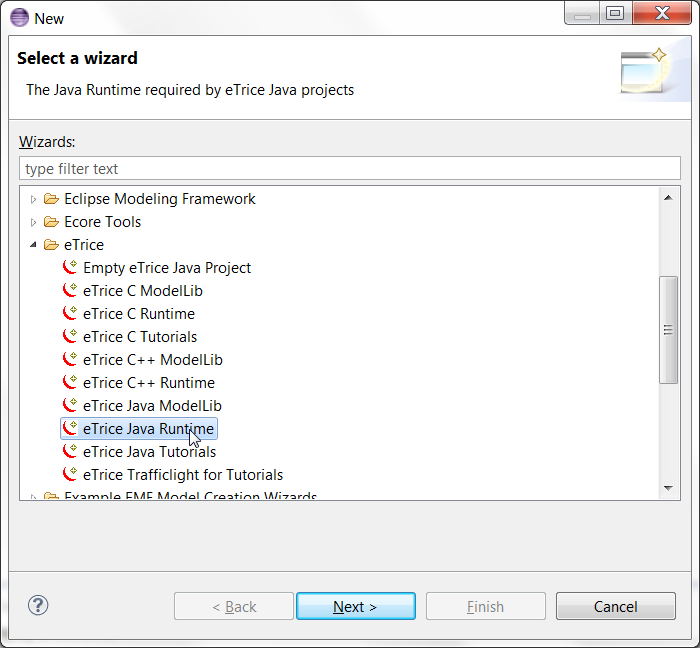
\includegraphics[width=0.8\textwidth]{images/013-SetupWorkspace03.png}
% !images/013-SetupWorkspace03.png!

Do the same steps for \textit{\eTrice{} Java Modellib} and \textit{\eTrice{} Java Tutorials}. To avoid temporary 
error markers you should keep the proposed order of installation. The resulting workspace should look like 
this:

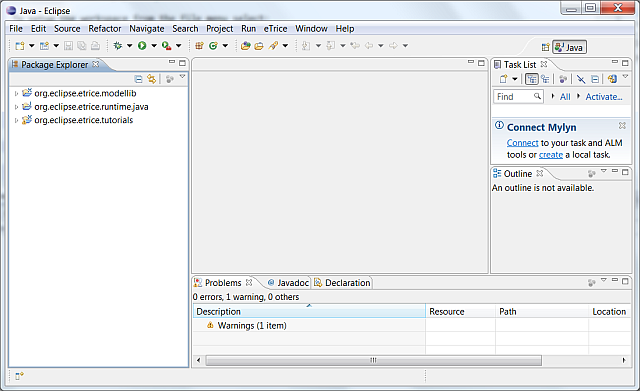
\includegraphics[width=0.8\textwidth]{images/013-SetupWorkspace04.png}
% !images/013-SetupWorkspace04.png!

Now workspace is set up and you can perform the tutorials or start with your work.

The tutorial models are available in the \textit{org.eclipse.etrice.tutorials.java} project. All tutorials are 
ready to generate and run without any changes. To start the code generator simply run 
\textbf{gen\_org.eclipse.etrice.tutorials.java.launch} as \textbf{gen\_org.eclipse.etrice.tutorials.java}: 

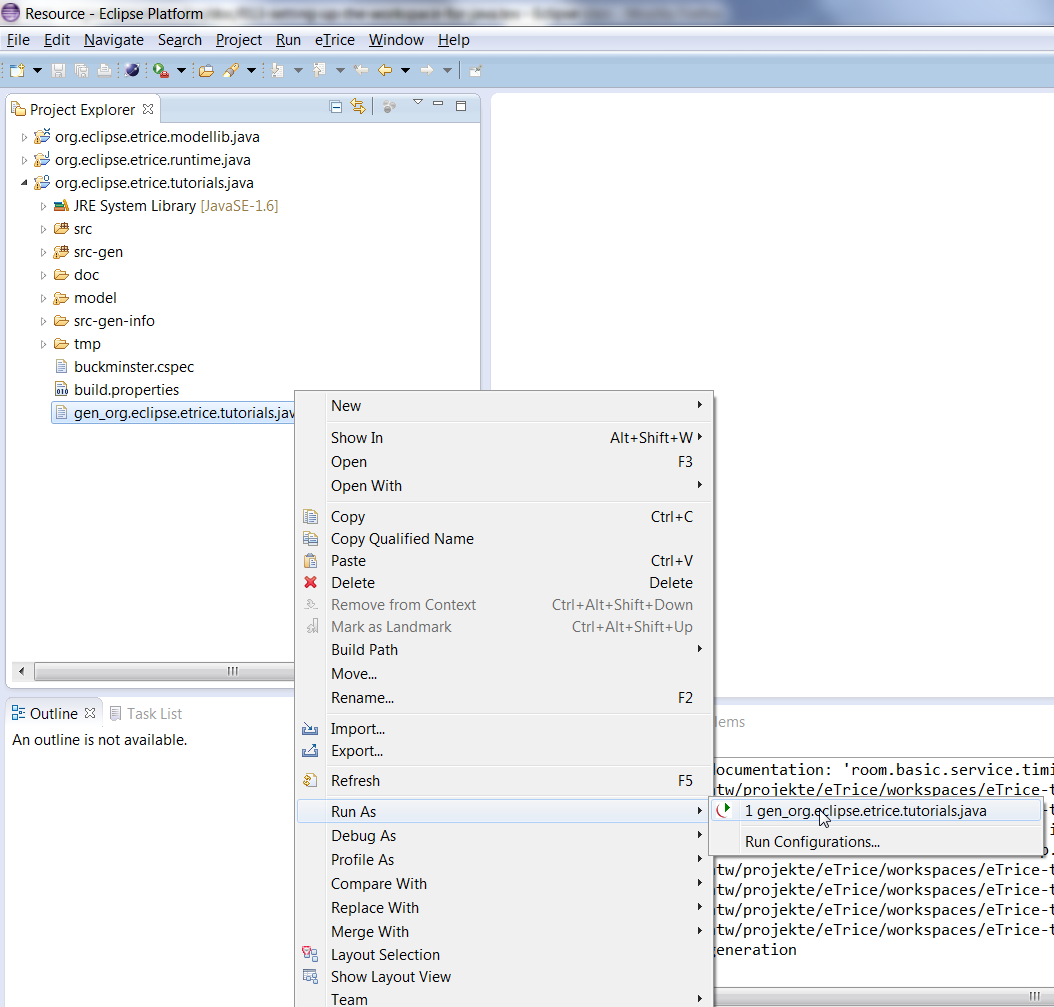
\includegraphics[width=0.8\textwidth]{images/013-SetupWorkspace05.png}
% !images/013-SetupWorkspace05.png!

The successful generation ends with \emph{Info: -- finished code generation} in the Console.

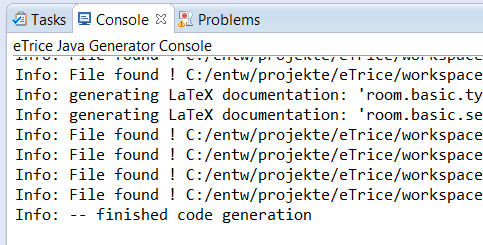
\includegraphics[width=0.8\textwidth]{images/013-SetupWorkspace051.png}
% !images/013-SetupWorkspace051.png!


For each tutorial in the folder src-gen a java package is generated including a java file called 
\textbf{SubSystem\_<Modelname>Runner.java} . To run the a generated application simply run this file as a java application:

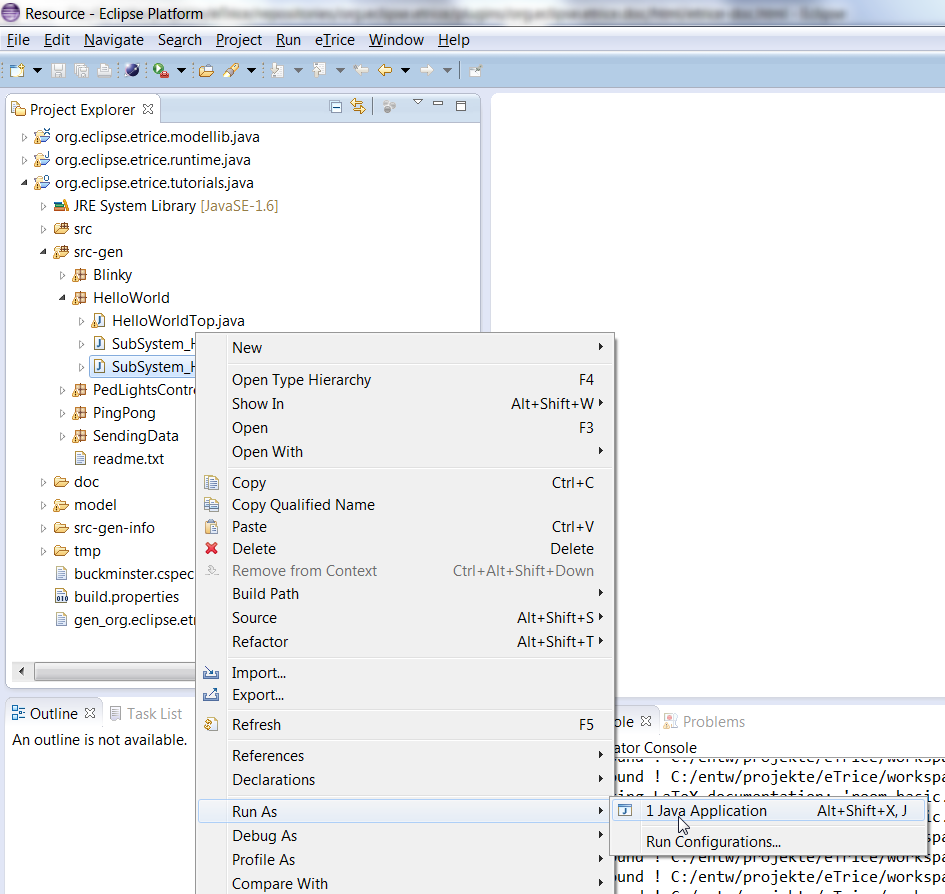
\includegraphics[width=0.8\textwidth]{images/013-SetupWorkspace06.png}
% !images/013-SetupWorkspace06.png!

To stop the application type \textit{quit} in the console window.
 
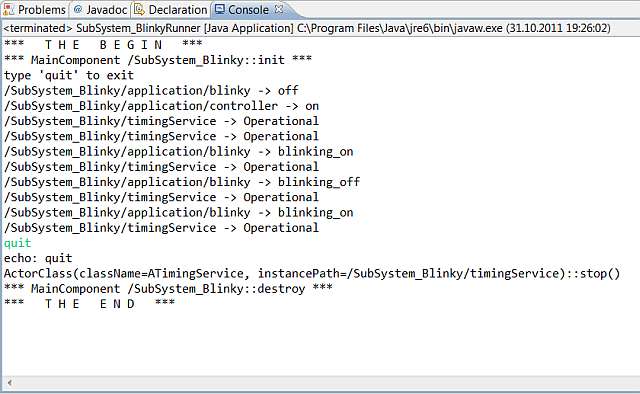
\includegraphics[width=0.8\textwidth]{images/013-SetupWorkspace07.png} 
% !images/013-SetupWorkspace07.png!

Performing the tutorials will setup a dedicated project for each tutorial. Therefore there are some 
slight changes especially whenever a path must be set (e.g. to the model library) within your own 
projects. All this is described in the tutorials.

\section{Setting up the Workspace for C Projects}

\textbf{Objectives for this tutorial:}
\begin{itemize}
	\item create all needed library projects (runtime.c and modellib.c)
	\item create the tutorial project with the examples
	\item create the project with a traffic light simulator
	\item test the workspace setup by running one of the examples
\end{itemize}

\subsection{Create Library, Tutorial and Simulator Projects}

Before you can start with C, some preconditions must be fulfilled:

\begin{itemize}
\item A C compiler must be installed on your machine. All tutorials are based on MinGW/GCC (Windows) and Posix/GCC (Linux), but currently only tested on Windows with MinGW/GCC
\item The CDT-Eclipse plugin must be installed as the C development environment.
\end{itemize}

After installation of eclipse and the \eTrice{} plug in, your workspace should look like this:  

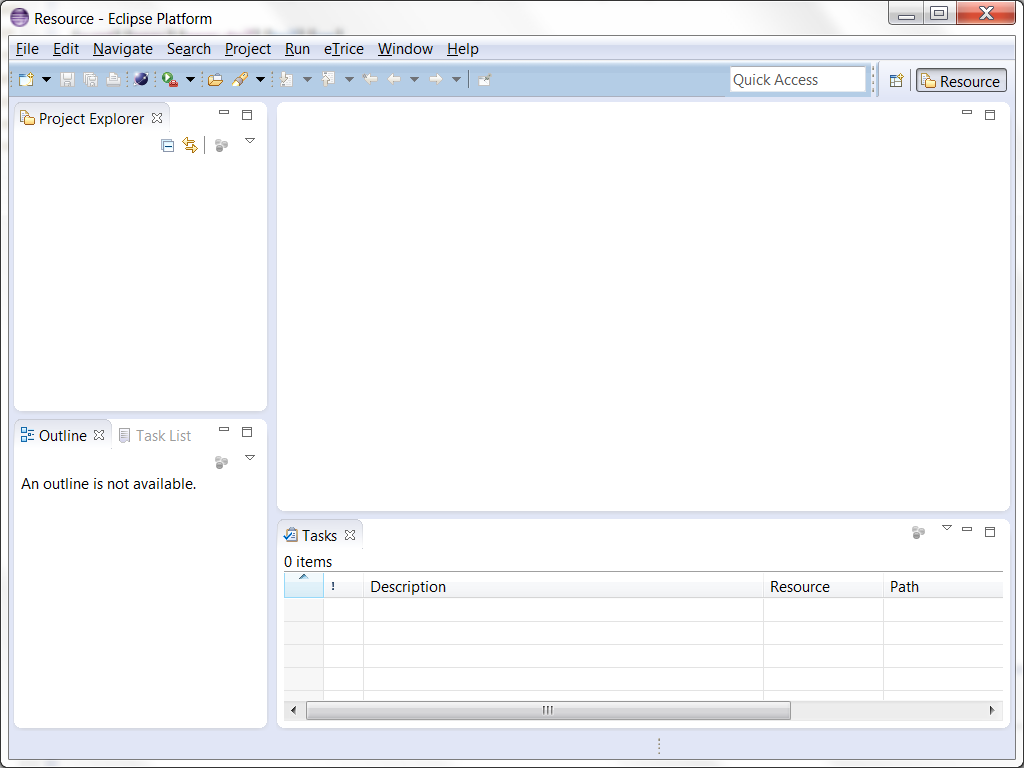
\includegraphics[width=0.8\textwidth]{images/013-SetupWorkspace01.png}
% !images/013-SetupWorkspace01.png!

Just the \eTrice{} menu item is visible of the installed \eTrice{} plugins.

\newpage
Select the menu \emph{File->New->Other}

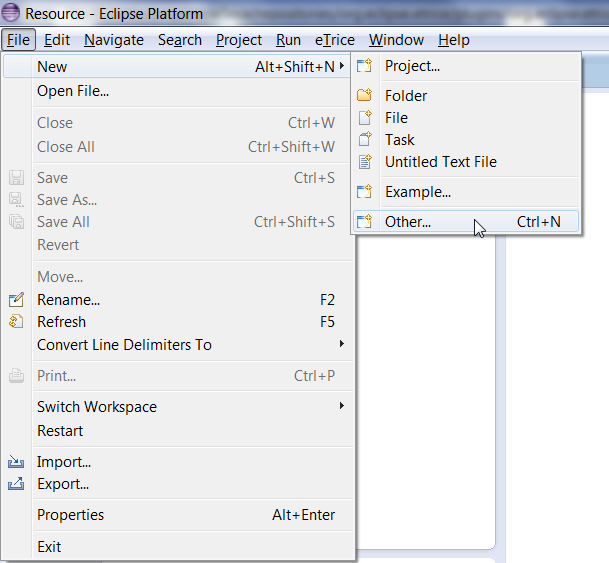
\includegraphics[width=0.6\textwidth]{images/013-SetupWorkspace02.png}
% !images/013-SetupWorkspace02.png!

Open the \emph{eTrice} tab and select \textit{eTrice C Runtime}

Press \emph{Next} and \emph{Finish} to install the Runtime into your workspace.

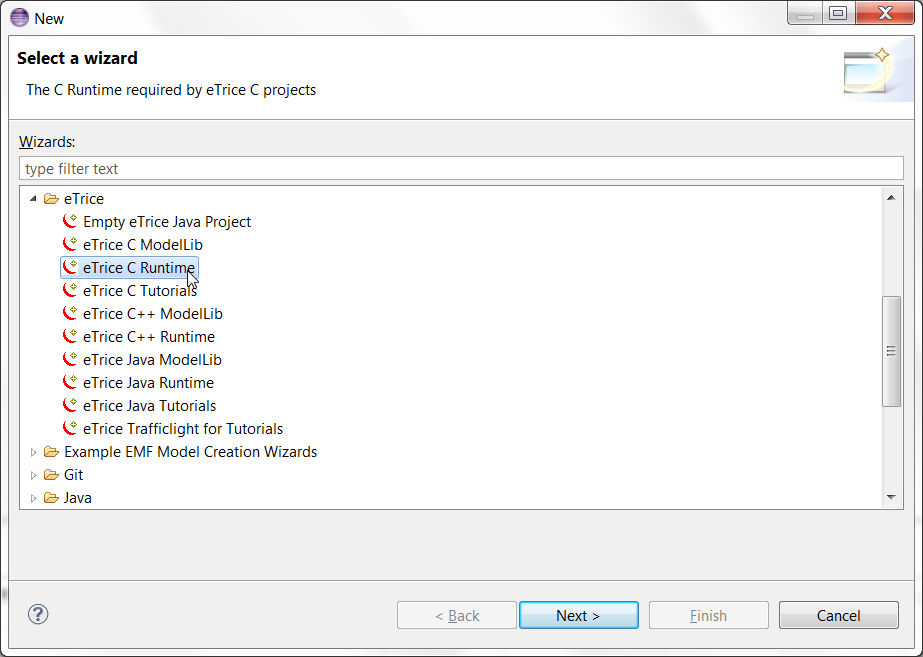
\includegraphics[width=0.6\textwidth]{images/014-SetupWorkspaceC005.png}
% !images/014-SetupWorkspaceC005.png!

\newpage
Do the same steps for \textit{eTrice C Modellib}, \textit{eTrice C Tutorials} and \textit{eTrice Trafficlight for Tutorials}. To avoid temporary 
error markers you should keep the proposed order of installation. The resulting workspace should look like 
this:

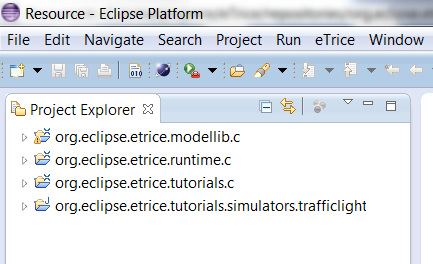
\includegraphics[width=0.5\textwidth]{images/014-SetupWorkspace007.png}
% !images/014-SetupWorkspace007.png!

\subsection{Perform Setup Test}

To check the correct setup of your workspace we run a little testproject contained in the tutorial project.

The tutorial models are available in the  \emph{org.eclipse.etrice.tutorials.c} project. All tutorials are ready to generate and run without any changes. To test the code generator and the workspace setup simply run 
\emph{gen\_SetupTestC.launch} as \emph{gen\_SetupTestC}: 

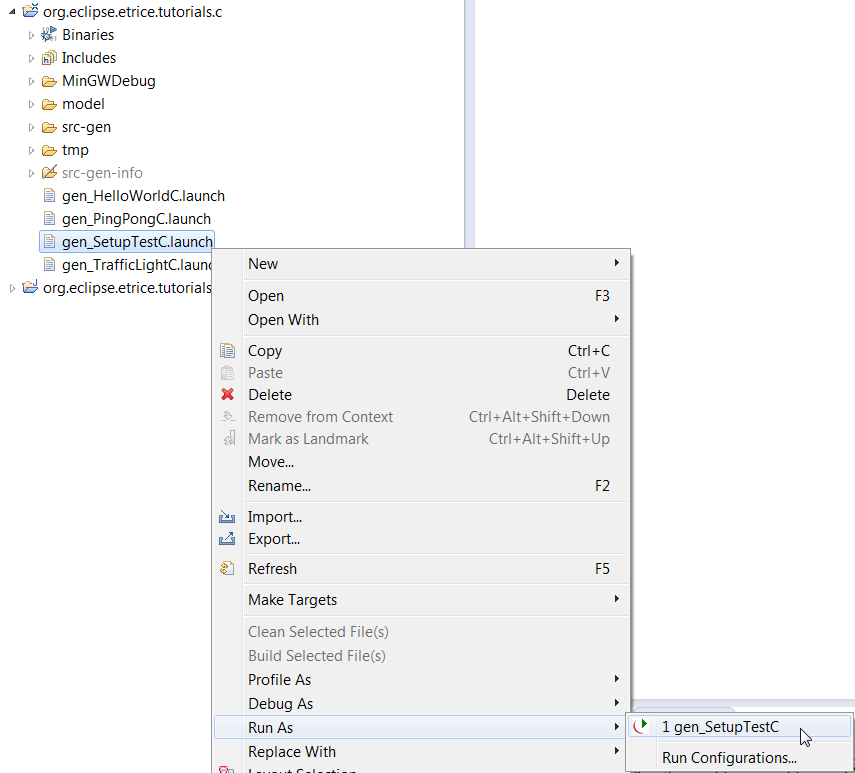
\includegraphics[width=0.6\textwidth]{images/014-05-gen_SetupTestC.png}
% !images/014-05-gen_SetupTestC.png!

\newpage
The successful generation ends with \emph{Info: -- finished code generation} in the Console.

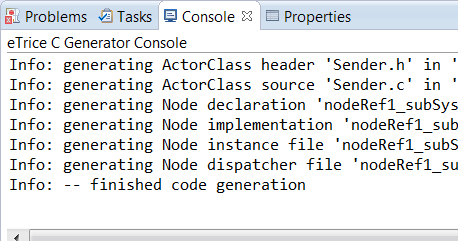
\includegraphics[width=0.5\textwidth]{images/014-06-FinishedCodeGeneration.png}
% !014-06-FinishedCodeGeneration.png!

For each tutorial in the folder src-gen a sub folder is generated which contains the generated code. The file \emph{<...>\_Runner.c} contains the main function. To run the generated application you first have to compile the project (with the hammer symbol in the C/C++ Perspective).

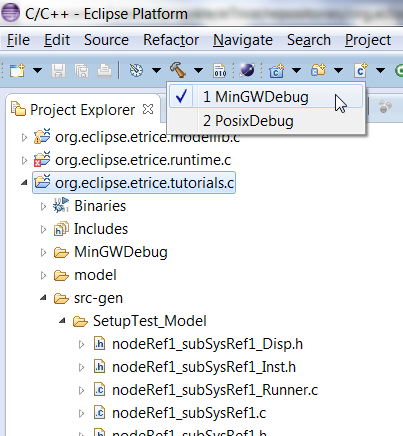
\includegraphics[width=0.5\textwidth]{images/014-07-Compile.png}
% !014-07-Compile.png!

If the compilitation does not succeed, make sure to clean and compile the projects \emph{org.eclipse.etrice.runtime.c} and \emph{org.eclipse.etrice.modellib.c} with the correct build configuration for your platform. Depending on the setup of your C compiler and CDT you might have to change the pre defined build configurations \emph{MinGWDebug} or \emph{PosixDebug}.

After the successful compilation you can run the application as \emph{Local C/C++ Application}.

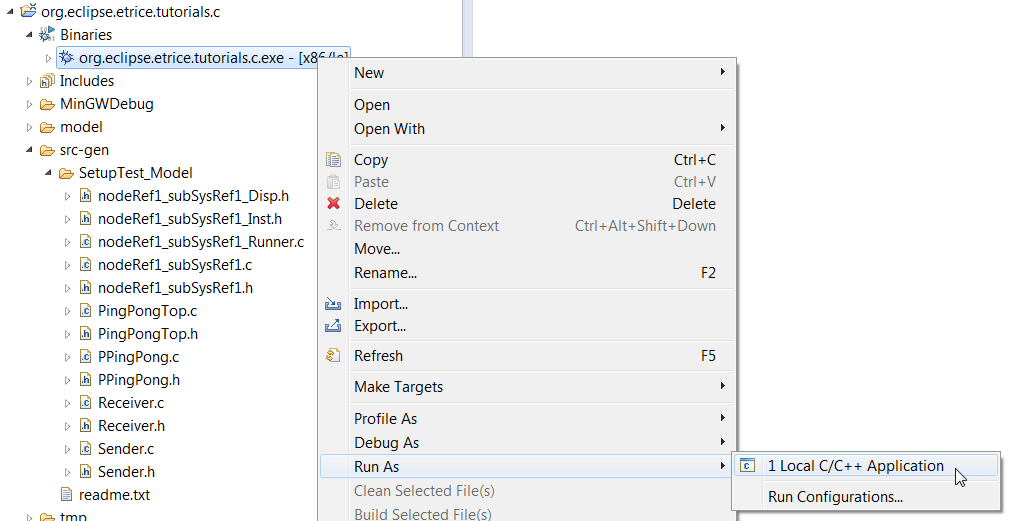
\includegraphics[width=0.7\textwidth]{images/014-08-RunAsC-CPP-Application.png}
% !images/014-08-RunAsC-CPP-Application.png!

\newpage
To stop the application type \emph{quit} in the console window. If your Console contains the lines
\begin{verbatim}
******************
*** Setup OK ***
******************
\end{verbatim}
your setup should be ok.

%TODO : update screenshot
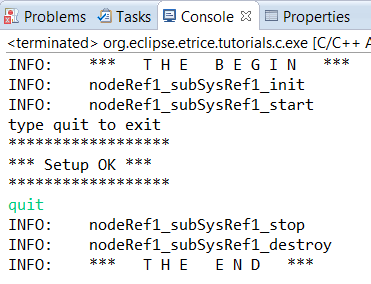
\includegraphics[width=0.5\textwidth]{images/014-09-ConsoleWithSetupOk.png} 
% !images/014-09-ConsoleWithSetupOk.png!

Now the workspace is set up and you can perform the tutorials or start with your work.


\section{HelloWorld for Java}

\subsection{Scope}

In this tutorial you will build your first very simple \eTrice{} model. The goal is to learn the work flow of 
\eTrice{} and to understand a few basic features of ROOM. You will perform the following steps:

\begin{enumerate}
\item create a new model from scratch
\item add a very simple state machine to an actor
\item generate the source code
\item run the model
\item open the message sequence chart
\end{enumerate}

Make sure that you have set up the workspace as described in \emph{Setting up the Workspace for Java}.

\subsection{Create a new model from scratch}

The easiest way to create a new \eTrice{} Project is to use the eclipse project wizard. From the eclipse file 
menu select \emph{File->New->Project} and create a new \emph{Empty eTrice Java Project} and name it \textbf{HelloWorld}.

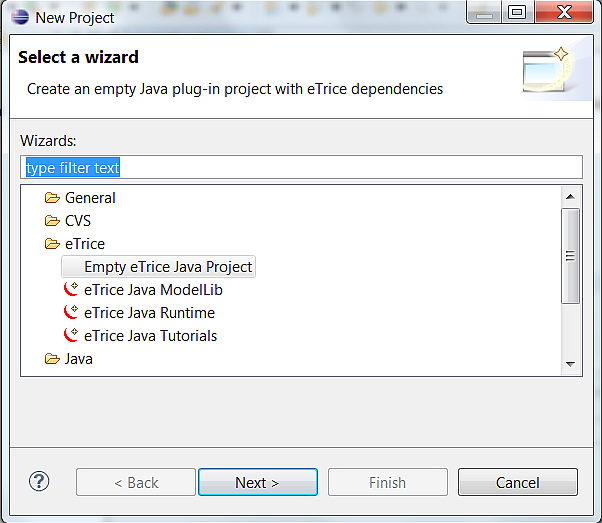
\includegraphics[width=0.8\textwidth]{images/015-HelloWorld10.png}

The wizard creates everything that is needed to create, build and run an \eTrice{} model. The resulting 
project should look like this:

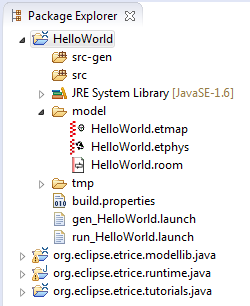
\includegraphics{images/015-HelloWorld11.png}

Within the model directory the model file \emph{HelloWorld.room} was created. Open the 
\emph{HelloWorld.room} file and delete the contents of the file. Open the content assist with Ctrl+Space 
and select \emph{RoomModel - model skeleton}.

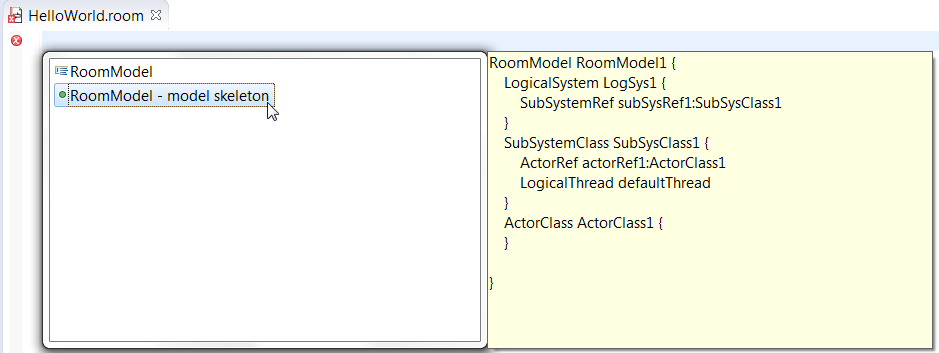
\includegraphics[width=0.6\textwidth]{images/015-HelloWorld12.png}

Edit the template variables by typing the new names and jumping with Tab from name to name.

The resulting model code should look like this:

\begin{lstlisting}[language=ROOM]
RoomModel HelloWorld_Model {

	LogicalSystem LogSys1 {
		SubSystemRef subSysRef1: SubSysClass1
	}

	SubSystemClass SubSysClass1 {
		ActorRef actorRef1: HelloWorldTop
		LogicalThread defaultThread
	}

	ActorClass HelloWorldTop { }

}
\end{lstlisting}

The physical model has already been created for us in file model/HelloWorld.etphys.
We can just leave it as it is.

\begin{lstlisting}[language=etPhys]
PhysicalModel PhysicalModel1 {

	PhysicalSystem PhysSys1 {
		NodeRef nodeRef1 : NodeClass1
	}

	NodeClass NodeClass1 {
		runtime = RuntimeClass1
		priomin = -10
		priomax = 10
		DefaultThread PhysicalThread1 {
			execmode = mixed
			interval = 100 ms
			prio = 0
			stacksize = 1024
			msgblocksize = 32
			msgpoolsize = 10
		}
	}

	RuntimeClass RuntimeClass1 {
		model = multiThreaded
	}
}
\end{lstlisting}

The physical model defines the setup of your nodes with their attributes like threads and mode of execution. In this case we define one node with one thread. 

Similar for the mapping model model/HelloWorld.etmap which is used to deploy the logical system onto the physical system.

\begin{lstlisting}[language=etMap]
MappingModel MappingModel1 {
	import HelloWorld_Model.* from "HelloWorldC.room"
	import PhysicalModel1.* from "HelloWorldC.etphys"
	Mapping LogSys1 -> PhysSys1 {
		SubSystemMapping subSysRef1 -> nodeRef1 {
			ThreadMapping defaultThread -> PhysicalThread1
		}
	}
}
\end{lstlisting}

The goal of \eTrice{} is to describe distributed systems on a logical level. In the current version not all 
elements will be used. But as prerequisite for further versions the following elements can be defined:
\begin{itemize}
\item the \textit{LogicalSystem} (currently optional)
\item at least one \textit{SubSystemClass} (mandatory)
\item at least one \textit{ActorClass} (mandatory)
\end{itemize}

The \textit{LogicalSystem} represents the complete distributed system and contains at least one 
\textit{SubSystemRef}. The \textit{SubSystemClass} represents an address space (e.g. a linux process or an image for a microcontroller) and contains at least one 
\textit{ActorRef}. The \textit{ActorClass} is the building block for building the hierachical structure of an application. 
A good point to start is to define a top level actor that can be used as structural root within the subsystem.

The outline view of the textual ROOM editor shows the main modeling elements in a navigation tree. You can jump to an element in the textual editor by double clicking the element in the outline view.

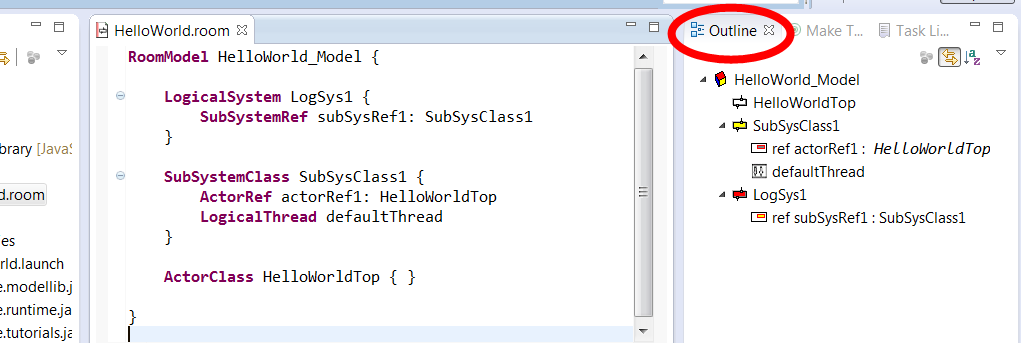
\includegraphics[width=0.8\textwidth]{images/015-HelloWorld02.png}
% !images/015-HelloWorld02.png!

\subsection{Create a state machine}

We will implement the Hello World code on the initial transition of the \textit{HelloWorldTop} actor. 
Therefore open the state machine editor by right clicking the \textit{HelloWorldTop} actor in the outline view and select \textit{Edit Behavior}.

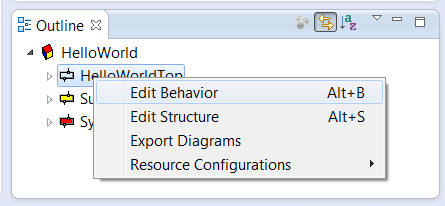
\includegraphics{images/015-HelloWorld03.png}
% !images/015-HelloWorld03.png!

The state machine editor will be opened. Drag and drop an \textit{Initial Point} from the tool box to the 
diagram into the top level state. Drag and drop a \textit{State} from the tool box to the diagram. Confirm the dialogue with \textit{ok}. Select the \textit{Transition} in the tool box and draw the transition from the \textit{Initial Point} to the State. Open the transition dialogue by double clicking the transition arrow and fill in the action code. Be aware of the different action code in Java and C.

\begin{figure}[ht]
\begin{minipage}[b]{0.45\linewidth}
	\begin{mdframed}
	\textbf{action code for Java}
	\begin{verbatim}
	System.out.println("Hello World !");
	\end{verbatim}
	\end{mdframed}
\end{minipage}
\hspace{0.5cm}
\begin{minipage}[b]{0.45\linewidth}
	\begin{mdframed}
	\textbf{action code for C}
	\begin{verbatim}
	printf("Hello World\n");
	\end{verbatim}
	\end{mdframed}
\end{minipage}
\end{figure}

 
The result should look like this:

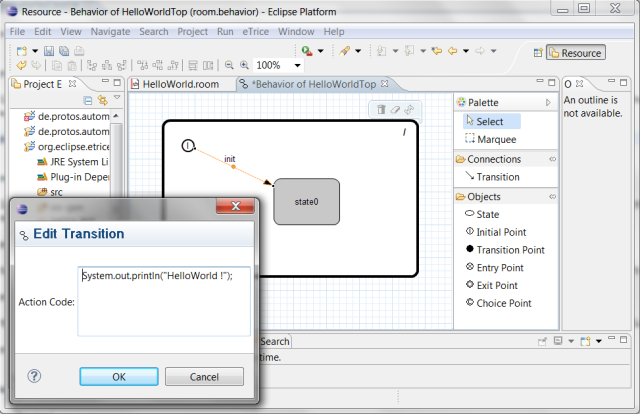
\includegraphics[width=0.8\textwidth]{images/015-HelloWorld04.png}
% !images/015-HelloWorld04.png!

Save the diagram and inspect the model (HelloWorld.room) file. Note that the textual representation was changed after saving 
the diagram.

\begin{figure}[ht]
\begin{minipage}[t]{0.50\linewidth}
\begin{mdframed}
	\textbf{room model for Java}
	\newline
\begin{lstlisting}[language=ROOM]
RoomModel HelloWorld_Model {
	LogicalSystem LogSys1 {
		SubSystemRef subSysRef1:SubSysClass1 
	}
	SubSystemClass SubSysClass1 {
		ActorRef actorRef1:HelloWorldTop 
		LogicalThread defaultThread
	}
	ActorClass HelloWorldTop {
		Structure { }
		Behavior {
			StateMachine {
				Transition init: initial -> state0 {
					action {
						"System.out.println(\"Hello World\");"
					}
				}
				State state0
			}
		}
	}
}
\end{lstlisting}
\end{mdframed}
\end{minipage}
\hspace{0.1cm}
\begin{minipage}[t]{0.50\linewidth}
\begin{mdframed}
	\textbf{room model for C}
	\newline
\begin{lstlisting}[language=ROOM]
RoomModel HelloWorld_Model {
	LogicalSystem LogSys1 {
		SubSystemRef subSysRef1: SubSysClass1
	}
	SubSystemClass SubSysClass1 {
		ActorRef actorRef1: HelloWorldTop
		LogicalThread defaultThread
	}
	ActorClass HelloWorldTop {
		Structure { }
		Behavior {
			StateMachine {
				Transition init: initial -> state0 {
					action {
						"printf(\"Hello World\\n\");"
					}
				}
				State state0
			}
		}
	}
}
\end{lstlisting}
\end{mdframed}
\end{minipage}
\end{figure}





\subsection{Build and run the model}

Now the model is finished and the source code can be generated. The project wizard has created a launch 
configuration that is responsible for generating the source code. In the project \textit{HelloWorld} right click \emph{gen\_HelloWorld.launch} and run it as \emph{gen\_HelloWorld}. 

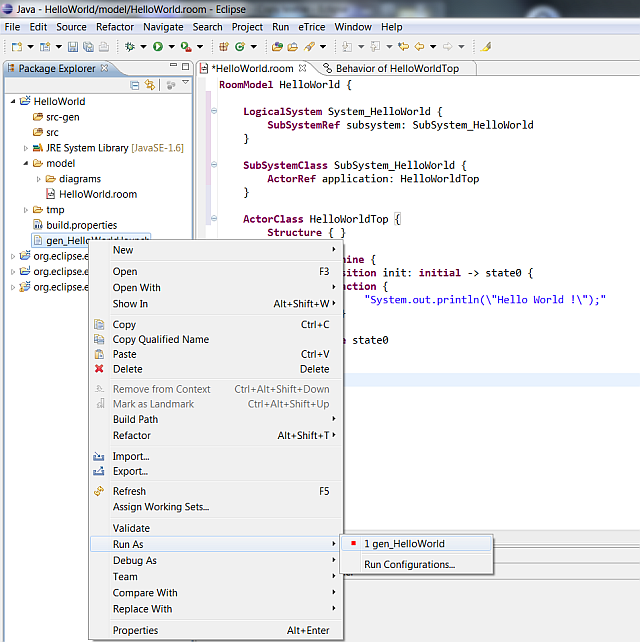
\includegraphics[width=0.8\textwidth]{images/015-HelloWorld06.png}

The source code for the model will be generated into the folder \emph{src-gen}. The main function will be contained in \emph{HelloWorld/Nod\_nodeRef1\_subSysRef1Runner.java}.
Select this file and run it as Java application or use the generated launch configuration \emph{run\_HelloWorld.launch}.

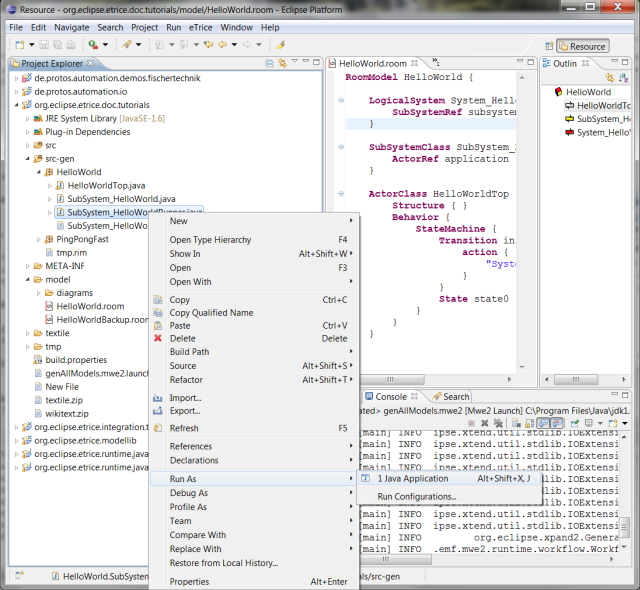
\includegraphics{images/015-HelloWorld07.png}


The Hello World application starts and the string \emph{"Hello World"} will be printed into the console window. To terminate the application the user must enter \emph{quit} in the console window.

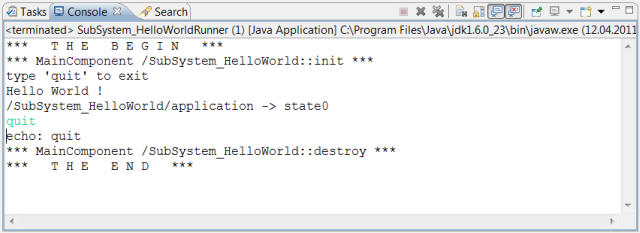
\includegraphics[width=0.6\textwidth]{images/015-HelloWorld08.png}

\subsection{Open the Message Sequence Chart}

For debugging and learning purposes, the application produced a Message Sequence Chart and wrote it to a file. Open the file \emph{subSysRef1\_Async.seq} or \emph{msc.seq} in the folder \emph{HelloWorld/tmp/log/} using the tool Trace2UML. Create the path if not already there.

Trace2UML is an open source MSC viewer and can be obtained here:
\begin{itemize}
\item \href{http://trace2uml.tigris.org/}{Trace2UML project home and download of windows version} 
\item \href{http://apt.astade.de/}{download of the Linux package of the Astade UML tool which contains Trace2UML}
\end{itemize}
After opening the file, you should see something like this:

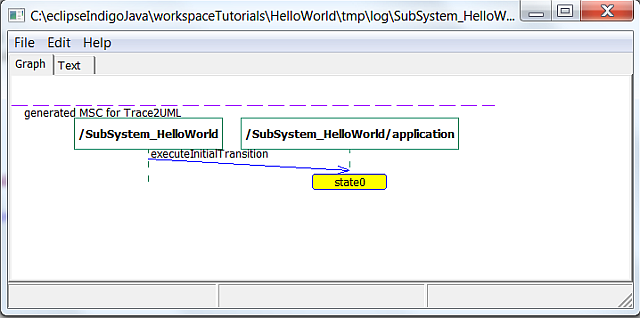
\includegraphics[width=0.6\textwidth]{images/015-HelloWorld09.png}
% !images/015-HelloWorld09.png!

The Actor with the instance path \emph{/LogSys1/subSysRef1/actorRef1} is in the state \emph{state0}. 
This is the simplest possible MSC. The MSCs for further tutorials will contain more information.


\subsection{Summary}

Now you have generated your first \eTrice{} model from scratch. You can switch between diagram editor and 
textual model representation (.room file) and you can see what will be generated during editing and saving the diagram files. 
You should take a look at the generated source files to understand how the state machine is generated and 
the life cycle of the application works. The next tutorials will deal with more complex hierarchies in structure and behavior.

\section{HelloWorld for C}

\subsection{Scope}

In this tutorial you will learn how to create a model for C from scratch. There are some more steps to do 
in C compared to Java. The goal is to get familiar with the additional steps. The Java tutorial is a 
prerequisite for the following explanations. 
You will perform the following steps:

\begin{enumerate}
\item create a new model from scratch for C
\item create structure and behavior similar to Java
\item create a launch configuration for the C code generator
\item setup the C environment
\item generate the source code
\item run the model
\end{enumerate}

Make sure that you have set up the workspace as described in \textit{Setting up the Workspace for C 
Projects}.


\subsection{Create a new model from scratch}

Before you can create a new C-model, you have to create a new C project as described in \textit{Setting up 
the Workspace for C Projects}.
Remember:
\begin{itemize}
\item select the \textit{C/C++} perspective
\item From the main menue select \textit{File->New->C Project}
\item Name the project \textit{HelloWorldC}
\item Project type is \textit{Executable / Empty C Project}
\item Toolchain is \textit{MinGW}
\end{itemize}

The workspace should look like this:

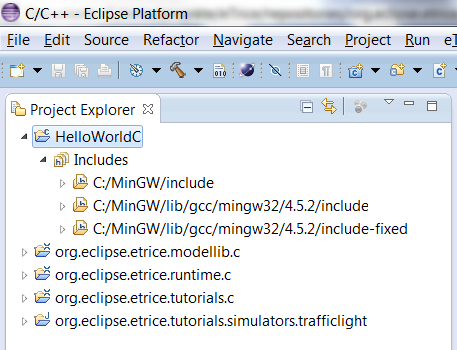
\includegraphics{images/016-HelloWorldC01.png}
% !images/016-HelloWorldC01.png!

The next step is to add the model folder:
Right click on the new project. Select \textit{New->Folder} and name it \textit{model}.

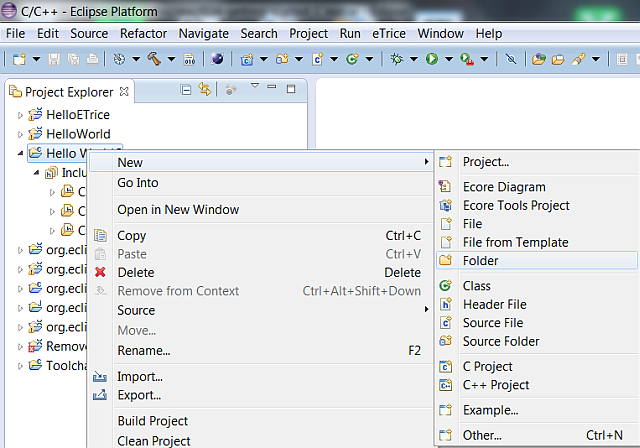
\includegraphics{images/016-HelloWorldC02.png}
% !images/016-HelloWorldC02.png!

Add the model file to the folder. Right click on the new folder. Select \textit{New->file} and name it 
\textit{HelloWorldC.room}.

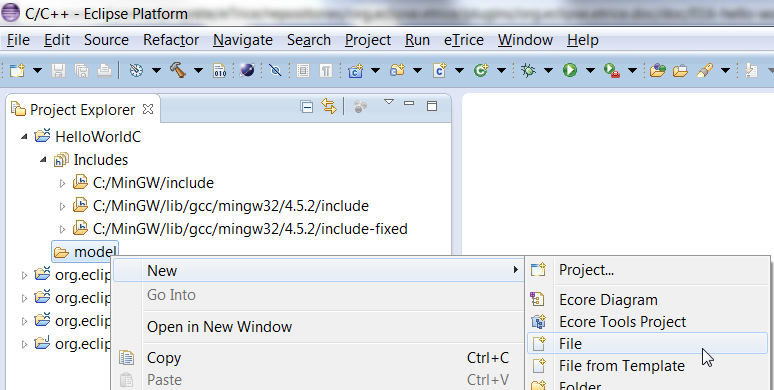
\includegraphics{images/016-HelloWorldC03.png}
% !images/016-HelloWorldC03.png!

Due to the file ending \textit{.room}, the tool will ask you to add the Xtext nature. Answer with 
\textit{Yes}. 

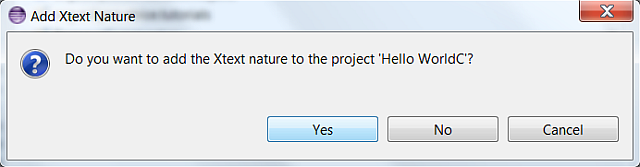
\includegraphics{images/016-HelloWorldC04.png}
% !images/016-HelloWorldC04.png!

The workspace should look like this:

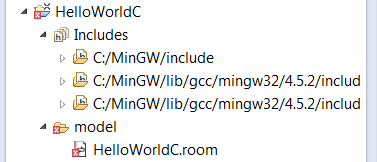
\includegraphics{images/016-HelloWorldC05.png}
% !images/016-HelloWorldC05.png!



\subsection{Create the HelloWorld model}

Once the model file is created and the Xtext nature is added, you can create the model as you did it for 
Java.
Creating the model is not the focus of this tutorial. Therefore copy and paste the following code into 
your model file. Optionally you can open and layout the diagrams.  
Recognize the C specific parts:
\begin{itemize}
\item The action code contains C instead of Java. Later versions will contain a common action language, 
but for the moment the action language is target specific.
\item The application must be shutdown on model level (see also \textit{etRuntimeConfig.h}).  
\end{itemize}

\begin{verbatim} 
RoomModel HelloWorldCModel {
	import room.basic.types.* from "../../org.eclipse.etrice.modellib.c/model/Types.room"
	SubSystemClass HelloWorldCSubSysClass {
		ActorRef HelloETriceTopRef:AHelloWorldCTop 
	}
	ActorClass AHelloWorldCTop {
		Structure { }
		Behavior {
			StateMachine {
				Transition init: initial -> state0 { }
				State state0 {
					entry {
						"printf(\"HelloWorldC !\\n\");"
						"SubSysClass_shutdown();"
						"\t\t\t\t\t\t"
					}
				}
			}
		}
	}	
}
\end{verbatim}

\subsection{Create a launch configuration to start the C code generator}

Other than in Java a launch configuration for the C code generator must be created.

From the \textit{Run} menu select \textit{Run Configurations}

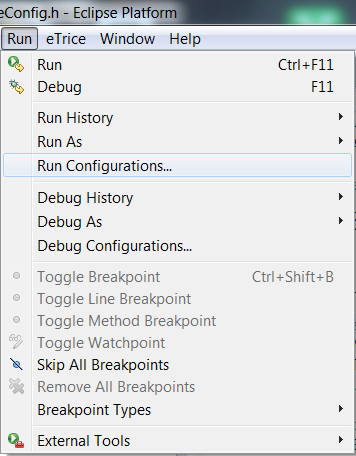
\includegraphics{images/016-HelloWorldC06.png}
% !images/016-HelloWorldC06.png!

Within the dialog select \textit{\eTrice{} C Generator} and click the \textit{New} button to create a new 
launch configuration.

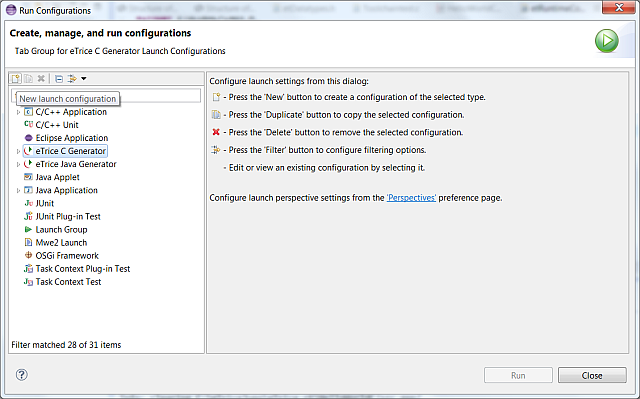
\includegraphics{images/016-HelloWorldC07.png}
% !images/016-HelloWorldC07.png!

A new configuration should be created. Name it \textit{gen\_HelloWorldC} and add the model via one of the 
\textit{add} buttons.

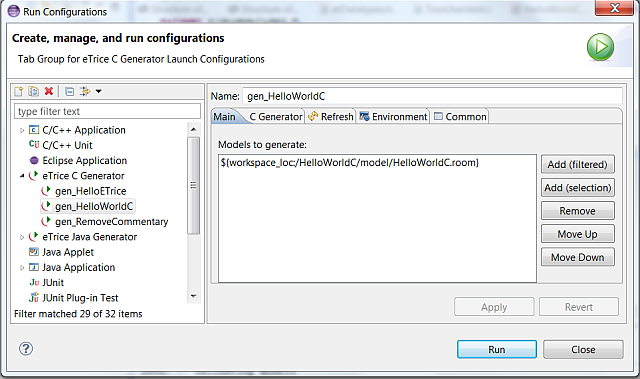
\includegraphics{images/016-HelloWorldC08.png}
% !images/016-HelloWorldC08.png!

In the \textit{Refresh} tab select \textit{The entire workspace} 

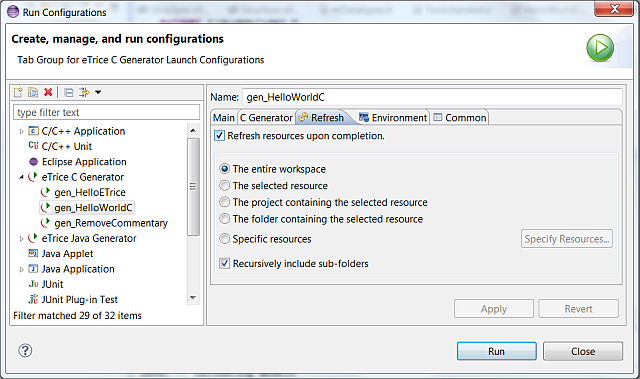
\includegraphics{images/016-HelloWorldC09.png}
% !images/016-HelloWorldC09.png!

In the \textit{Common} tab select \textit{Shared file} and add the \textit{HelloWorldC} project via the 
\textit{Browse} button.

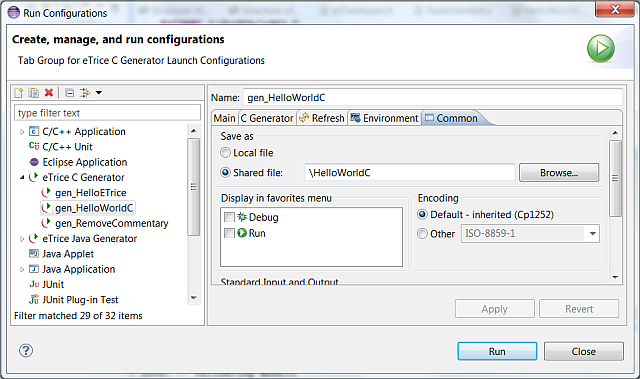
\includegraphics{images/016-HelloWorldC10.png}
% !images/016-HelloWorldC10.png!

Apply your changes. The new configuration should now exist in your workspace.

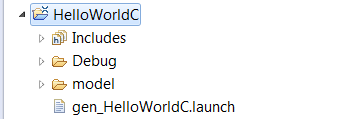
\includegraphics{images/016-HelloWorldC11.png}
% !images/016-HelloWorldC11.png!


\subsection{Generate the code}

Now you can generate the code as you know it from Java. Right click on the launch configuration and run it 
as \textit{gen\_HelloWorldC}.

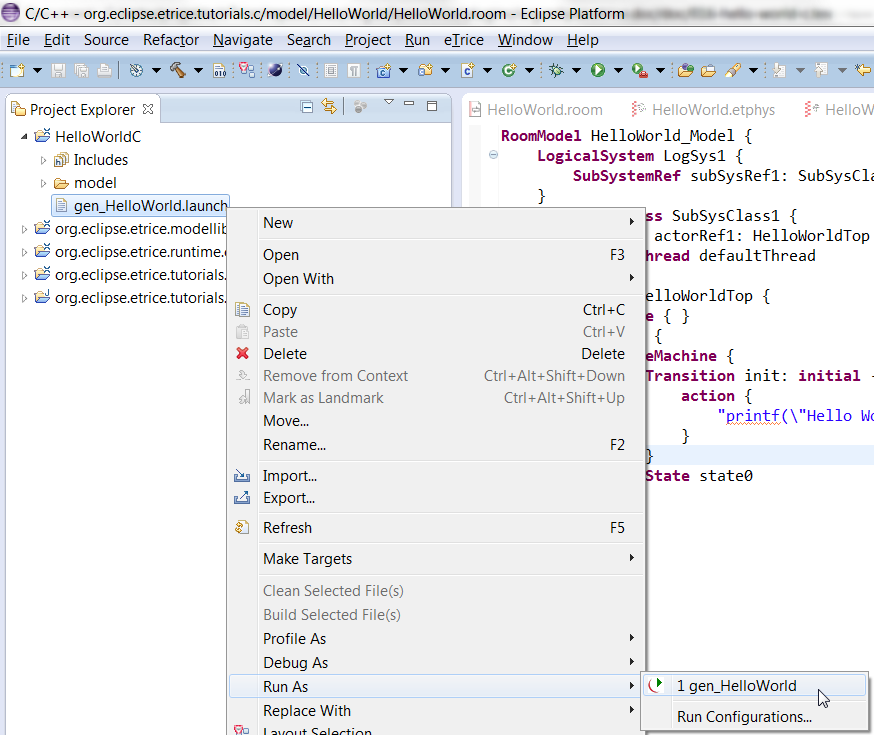
\includegraphics{images/016-HelloWorldC12.png}
% !images/016-HelloWorldC12.png!

The code should be generated.

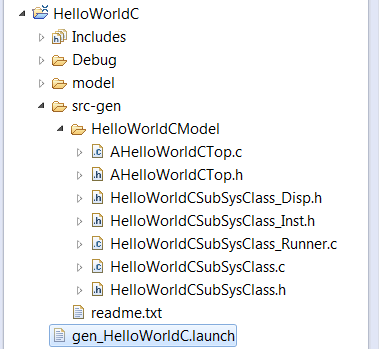
\includegraphics{images/016-HelloWorldC13.png}
% !images/016-HelloWorldC13.png!

\subsection{Setup the include path}

Before you can build the application you must setup the include path for the runtime system. Right click 
the project and select \textit{Properties}. Add the include path as described in \textit{setting up the 
workspace}.

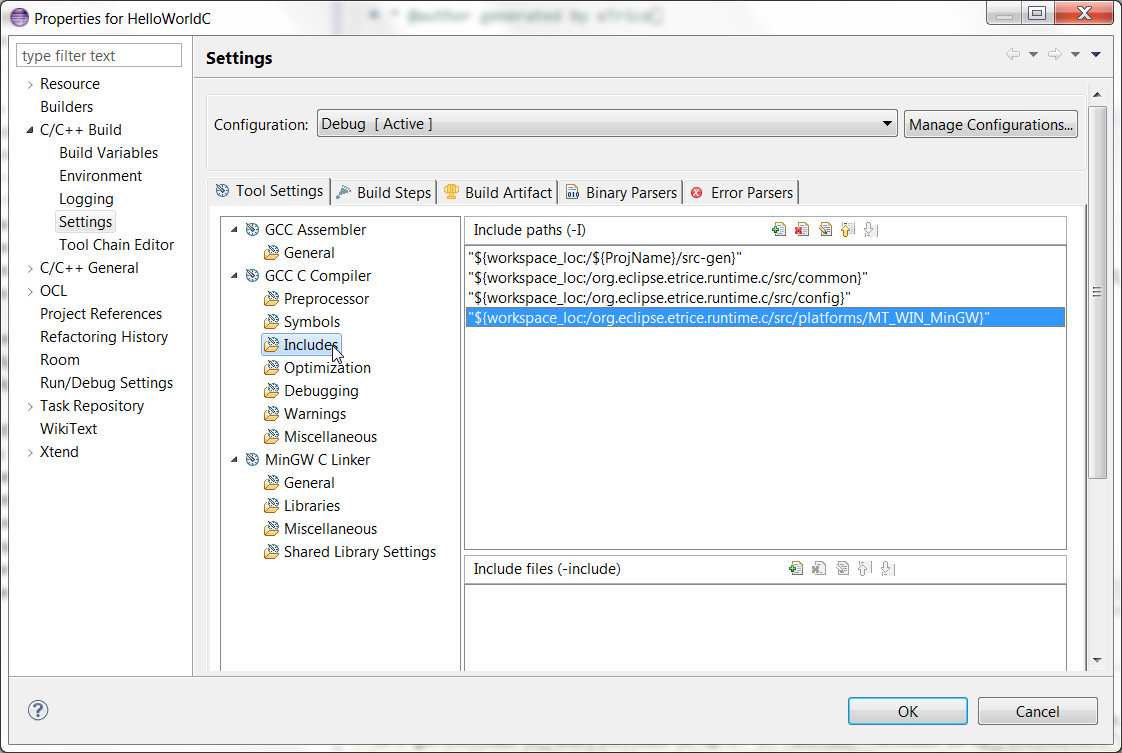
\includegraphics{images/016-HelloWorldC14.png}
% !images/016-HelloWorldC14.png!

Add the runtime library.

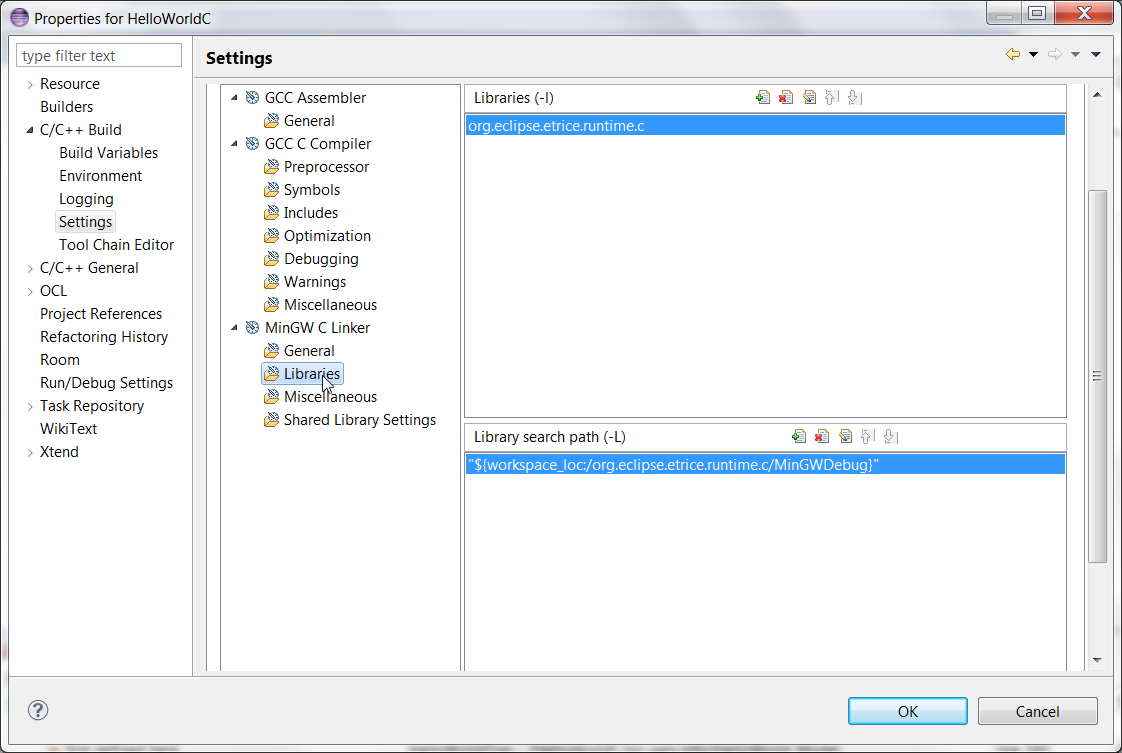
\includegraphics{images/016-HelloWorldC15.png}
% !images/016-HelloWorldC15!

Recognize the name of the library ("org.eclipse.etrice.runtime.c"). The library file on your disk is 
"liborg.eclipse.etrice.runtime.c.a". 

\subsection{Build and run the model}

Now you can build the application. Click the build button to build the application.
Run the application as \textit{Local C/C++ Application}.
Verify the output.

\includegraphics{images/016-HelloWorldC16.png}
% !images/016-HelloWorldC16.png!

\subsection{Summary}

You are now familiar with all necessary steps to create, build and run an \eTrice{} C model from scratch. You 
are able to create a launch configuration to start the code generator and to perform all necessary 
settings to compile and link the application.  

The next tutorial provides an exercise to get more familiar with these working steps.

\section{Ping Pong Tutorial (Java and C)}
\label{sec:ping_pong_tutorial}

\subsection{Scope}

This tutorial describes how to create a simple hierarchical actor system of actors communicating via ports and bindings. 
Additionally you will use the Timing Service from the eTrice model library.
This tutorial can be done for the target languages Java or C.
For the Ping Pong scenario we want to create a model with a sender and a reveiver of a message. The receiver has to wait for the ping message from the sender, wait for a second and respond with a pong message.

The resulting Message Sequence Chart (MSC) at the ende of this tutorial should look like this:

\includegraphics[width=0.8\textwidth]{images/017-01-MSC.png}

We will take this MSC as specification for the desired behavior.

You will perform the following steps:

\begin{enumerate}
\item create a new model from scratch
\item define a protocol
\item create an actor structure
\item create finite state machines
\item use the predefined \textit{TimingService}
\item build and run the model
\item open the message sequence chart
\end{enumerate}

\subsection{Create a new model from scratch}

Create a new \eTrice{} project according to \textit{HelloWorld for Java or C} and name it \textit{PingPong}.

Your \emph{ROOM} model should look like this:

\begin{lstlisting}[language=ROOM]
RoomModel PingPong_Model {
	LogicalSystem LogSys1 {
		SubSystemRef subSysRef1:SubSysClass1 
	}
	SubSystemClass SubSysClass1 {
		ActorRef actorRef1:PingPongTop 
		LogicalThread defaultThread
	}
	ActorClass PingPongTop {
	}
}
\end{lstlisting}

\subsection{Create a new protocol}

First we define a protocol for the communication between the Sender and the Receiver. From the specification MSC above we can derive that the Sender sends a \emph{ping} message to the receiver and the receiver responds with a \emph{pong} message. 

In \emph{ROOM} the \emph{ProtocolClass} specifies interfaces. In this case we go for an asynchronous, bidirectional messaging interface (eventdriven) which is the standard communication type for a \emph{ProtocolClass}.
With the help of \textit{Content Assist} (Ctrl+Space) we create a \textit{ProtocolClass} and name it 
\textit{PingPongProtocol}.
Inside the brackets use the \textit{Content Assist}  to create two incoming messages called 
\textit{ping} and \textit{pong}.

The resulting code should look like this:

\begin{lstlisting}[language=ROOM]
	ProtocolClass PingPongProtocol {
		incoming {
			Message ping()
		}
		outgoing {
			Message pong()
		}
	} 
\end{lstlisting}

With \emph{Ctrl-Shift+F} or selecting \textit{Format} from the context menu you can format the \emph{ROOM} model. Note that 
the new \textit{ProtocolClass} is displayed in the outline view.

\subsection{Create the Actor Structure}
\subsubsection*{Add two additional actor classes}

Position the cursor outside any class definition and call the \textit{Content Assist} with \emph{Ctrl+Space}.
Select \textit{ActorClass - actor class skeleton or ActorClass} and name the ActorClass \textit{Sender}.

\includegraphics[width=0.6\textwidth]{images/017-02-content-assist.png}
% !images/017-02-content-assist.png!

Repeat the described procedure and name the new actor \textit{Receiver}.

With Ctrl+Shift+F you can format your textual model. 

The Result:

\begin{lstlisting}[language=ROOM]
RoomModel PingPong_Model {

	LogicalSystem LogSys1 {
		SubSystemRef subSysRef1: SubSysClass1
	}

	SubSystemClass SubSysClass1 {
		ActorRef actorRef1: PingPongTop
		LogicalThread defaultThread
	}

	ActorClass PingPongTop { }

	ActorClass Sender { }

	ActorClass Receiver { }

}
\end{lstlisting}

You can should also see the new \emph{ActorClass}es in the outline view.

\subsubsection*{Add ports to the actors}

To open the graphical structure editor, right click \textit{Receiver} in the Outline View and select \textit{Edit Structure}. Drag and Drop an 
\textit{Interface Port} from the \emph{Palette} to the border of the \textit{Receiver} actor. Note that an \emph{Interface Port} can only be placed on the border of the actor. Name the port \textit{sender} and select \textit{PingPongProtocol} as Protocol from the drop down list. The checkboxes \textit{Conjugated} and \textit{Is Relay Port} stay unchecked. Click \textit{ok}. The 
resulting structure should look like this:

\includegraphics[width=0.6\textwidth]{images/017-04-Port-for-Actor-Receiver.png}
% !images/017-04-Port-for-Actor-Receiver.png!

Repeat the steps above for the \textit{sender}. Create a port named \emph{receiver} with the same \emph{Protocol} and make it \emph{Conjugated}.

Keep in mind that the protocol defines \textit{ping} as incoming message and \textit{pong} as outgoing message. 
\textit{Receiver} receives \emph{ping} and sends \emph{pong}. Therefore the \textit{Receiver}s port must be a 
regular port. The \textit{Sender} has to send \textit{ping} and receive \textit{pong}. Therefore the \textit{Sender}s port must be a conjugated port.

\subsubsection*{Build hierarchical actor structure}

Now we want to add the new actors to the structure of \emph{ActorClass} \emph{PingPongTop}.

From the outline view right click \textit{PingPongTop} and select \textit{Edit Structure}. Remember that you can only see the outline view if the textual editor with the .room file is active.

Drag and Drop an \textit{ActorRef} inside the \textit{PingPongTop} actor. Name it \textit{sender}. From the actor class drop down list select \textit{Sender}. Do the same for \textit{Receiver}. Connect the ports 
via the binding tool int the \emph{Palette}. The resulting structure should look like this:

\includegraphics[width=0.8\textwidth]{images/017-03-PingPongTop-Structure.png}
% !images/017-03-PingPongTop-Structure.png!

We have build the structure of a hierarchical actor system with two actors that send each other messages.

\subsubsection*{Import the Timing Service}

In order to implement the waiting time of the \emph{Receiver} we need a timing service. The timing service is provided by the model library and must be imported before it can be used in your model.

\begin{figure}[ht]
\begin{minipage}[t]{0.50\linewidth}
\begin{mdframed}
	\textbf{room model for Java}
	\newline
\begin{lstlisting}[language=ROOM]
RoomModel PingPong_Model {

	import room.basic.service.timing.* from "../../org.eclipse.etrice.modellib.java/model/TimingService.room"
	(...)
\end{lstlisting}
\end{mdframed}
\end{minipage}
\hspace{0.1cm}
\begin{minipage}[t]{0.50\linewidth}
\begin{mdframed}
	\textbf{room model for C}
	\newline
\begin{lstlisting}[language=ROOM]
RoomModel PingPong_Model {

	import room.basic.service.timing.* from "../../org.eclipse.etrice.modellib.c/model/TimingService.room"
	(...)
\end{lstlisting}
\end{mdframed}
\end{minipage}
\end{figure}

This is the first time you use an element from the modellib. Make sure that your Java Build Path or the settings for your C compiler are configured to use the modellib. Otherwise the generated code can not be built.

\begin{figure}[ht]
\begin{minipage}[t]{0.50\linewidth}
\begin{mdframed}
	\textbf{build settings for Java}
	\newline
Right click the project \textit{PingPong} and select \emph{Properties -> Java Build Path -> Projects} . Add the project \emph{org.eclipse.etrice.modellib.java} .
  
\includegraphics[width=0.8\textwidth]{images/020-Blinky16.png}
% !images/020-Blinky16.png! 

\end{mdframed}
\end{minipage}
\hspace{0.1cm}
\begin{minipage}[t]{0.50\linewidth}
\begin{mdframed}
	\textbf{build settings for C}
	\newline

Right click the project \textit{PingPong} and select \emph{Properties -> C/C++ Build -> Settings -> Includes}. Add the include path \emph{org.eclipse.etrice.modellib.c/src-gen} to the list.

\includegraphics[width=0.8\textwidth]{images/017-06-Settings-for-C-Includes.png}
% !images/017-06-Settings-for-C-Includes.png! 

Select \emph{Properties -> C/C++ Build -> Settings -> Libraries}. Add the library \emph{org.eclipse.etrice.modellib.c} and the library path 
\emph{org.eclipse.etrice.modellib.c/MinGWDebug} to the lists. For Posix the path will be \emph{org.eclipse.etrice.modellib.c/PosixDebug}.
	
\includegraphics[width=0.8\textwidth]{images/017-07-Settings-for-C-Libraries.png}
% !images/017-07-Settings-for-C-Libraries.png! 

\end{mdframed}
\end{minipage}
\end{figure}

Now the imported library can be used within your model and we will add the actor with the timing service to our model.

Right click the \emph{SubSystemClass} \emph{SubSysClass1} in the outline view and select \textit{Edit Structure}. The \emph{ActorClass} \emph{PingPongTop} is already referenced in the subsystem as \textit{actorRef1}. Drag and 
Drop an \textit{ActorRef} into the structure of \emph{SubSysClass1} and name it \textit{timingService}. From the actor class drop down list select \textit{room.basic.service.timing.ATimingService}. Draw a 
\textit{LayerConnection} from \textit{actorRef1} to the service provision point (\emph{SPP}) of the 
\textit{timingService}. The resulting structure should look like this:

\includegraphics[width=0.8\textwidth]{images/017-08-SubSystem-with-timing-service.png}
% !017-08-SubSystem-with-timing-service.png! 

The layer connection between an \emph{ActorRef} and a \emph{SPP} enables the use of service access points (\emph{SAP}) for the service provided by the \emph{SPP}, in this case the timing service. \emph{SAP}s and \emph{SPP}s are ports with a different kind of connection. Every \emph{SAP} of the type \emph{PTimer} inside actorRef1 is now connected automatically by the code generator with the \emph{SPP} of the \emph{timingService}.

The current version of \eTrice{} does not provide a graphical element for a service access point (SAP). 
Therefore the SAPs to access the timing service must be added in the .room file. Open the 
\textit{PingPong.room} file and navigate to the \textit{Receiver} actor. Add the SAP for the protocol \emph{PTimer} to the structure of the actor:

\begin{lstlisting}[language=ROOM]
	ActorClass Receiver {
		Interface {
			Port sender: PingPongProtocol
		}
		Structure {
			external Port sender
			SAP timing : PTimer
		}
	}
\end{lstlisting}

Now the \emph{Receiver} can use the timing service.

\subsubsection*{Inspect the Actor Structure}
Before we start with the implementation of the behavior we will have a short look at the instance tree of the application we built so far:

\includegraphics[width=0.4\textwidth]{images/017-09-PingPong_InstanceTree.jpg}
% !017-09-PingPong_InstanceTree.jpg! 

For each instance you can see the names of the \emph{ActorRef}s and in brackets the names of the \emph{ActorClass}es. Starting at the subsystem level this instance tree will be implemented by the code generator. The subsystem will be implemented as process in Linux or Windows.


\subsection{Implement the Behavior}

We will implement two finite state machines (\emph{FSM}s) to  define the event driven behavior of the actors  \emph{Sender} and \emph{Receiver}.

Before you start with the implementation, have a look at the MSC with the specification of the behavior.

Lets start with the \emph{Sender}. Right click to \emph{Sender} in the outline view or the structure editor and select \emph{Edit Behavior}.
Drag and Drop the \textit{Initial Point} and two \textit{States} into the top state. Name the states 
\textit{SendingPing} and \textit{ReceivedPong}. 
Use the \textit{Transition} tool to draw transitions from \textit{init} to \textit{SendingPing} and from \textit{SendingPing} to \textit{ReceivedPong}.
When you draw a transition, the Dialog \emph{Edit Transition} opens. Here you can specify the trigger event and the action code for each transition. Note that the initial transition does not have a trigger event.
The transition dialog for the Transition from \textit{SendingPing} to \textit{ReceivedPong} should look like this:

\includegraphics[width=0.6\textwidth]{images/017-10-Edit-Transition.png}
% !images/017-10-Edit-Transition.png! 

The transition will now be triggered by an incoming message \emph{ping} at the port \emph{receiver}.

Now we open the dialog \emph{Edit State} of the state \textit{SendingPing} by right clicking the state and selecting \emph{Edit State} from the menu.
We want to send the message \emph{ping} in the entry code of this state.
The defined ports will be generated as a member attribute of the actor class from type of the attached 
protocol. To send a message you must state \textit{port.message(param);}. In this example 
\textit{receiver.ping();} sends the \textit{ping} message via the \textit{receiver} port. You can also use the Button \emph{Messages} to select the message from the list of available ports and their available messages.
Assuming that the actor \textit{Receiver} is connected to this port, the message will be sent there.

The FSM of \emph{Sender} should now look like this:

\includegraphics[width=0.8\textwidth]{images/017-11-FSM-Sender.png}
% !images/017-11-FSM-Sender.png!

Now we implement the FSM of the \emph{ActorClass} \emph{Receiver}.

\includegraphics[width=0.8\textwidth]{images/017-12-FSM-Receiver.png}
% !images/017-12-FSM-Receiver.png!

In the entry code of the state \emph{WaitingForAWhile} we start the timeout: 

\begin{verbatim}
timing.startTimeout(1000);
\end{verbatim}

In the entry code of the state \emph{SentPong} we send the message \emph{pong} back to the \emph{Sender}: 

\begin{verbatim}
sender.pong();
\end{verbatim}

Save the diagram and inspect the \emph{PingPong.room} file. The \emph{Receiver} should look like this:

\begin{lstlisting}[language=ROOM]
	ActorClass Receiver {
		Interface {
			Port sender: PingPongProtocol
		}
		Structure {
			external Port sender
			SAP timing : PTimer
		}
		Behavior {
			StateMachine {
				Transition init: initial -> WaitingForPing { }
				Transition tr0: WaitingForPing -> WaitingForAWhile {
					triggers {
						<ping: sender>
					}
				}
				Transition tr1: WaitingForAWhile -> SentPong {
					triggers {
						<timeout: timing>
					}
				}
				State WaitingForPing
				State SentPong {
					entry {
						"sender.pong();"
					}
				}
				State WaitingForAWhile {
					entry {
						"timing.startTimeout(1000);"
					}
				}
			}
		}
	}
\end{lstlisting}

The PingPong model is done now. You can generate, compile and run it as described in \emph{Hello World for C} or \emph{Hello World for Java}. The generated MSC in tmp/log should show the same MSC we used to specify the behavior at the beginning of this tutorial.

\includegraphics[width=0.8\textwidth]{images/017-01-MSC.png}
% !images/017-01-MSC.png!

Please note that the timeout messages startTimeout and timeout might vary depending on the target language and are not displayed completely correct in the current version (red dot). The MSC logger will be extended to handle this correct in the next version.

\subsection{Summary}

Within this tutorial you have learned how to create a FSM with transitions triggered by incoming messages. You have used entry code to send messages and have used the timing service from the model library. You are now familiar with the basic features of \eTrice{}. Further tutorials and examples will take this knowledge as a precondition.

\section{Traffic Light}

\subsection{Scope}

In this tutorial you will build an example with a more advanced state machine.
To make it more appealing we've added a little GUI with two traffic lights, one for the cars and one for pedestrians.
The GUI also contains a button that can be used to request green for pedestrians.

You will perform the following steps:

\begin{enumerate}
\item create a new model from scratch
\item create a pedestrian light actor
\item perform a first test
\item implement the behavior
\item do some configuration
\end{enumerate}

\subsection{Create a new model from scratch}

The easiest way to create a new \eTrice{} Project is to use the eclipse project wizard. From the eclipse file 
menu select \emph{File->New->Project} and create a new \emph{Empty eTrice Java Project} and name it \textbf{TrafficLight}.

In the model directory locate TrafficLight.room and edit it. We only rename a little.
The model should look like this:

\begin{lstlisting}[language=ROOM]
RoomModel TrafficLight {

	LogicalSystem TrafficLight {
		SubSystemRef main: Main
	}

	SubSystemClass Main {
		ActorRef pedLight: PedestrianLight
		LogicalThread defaultThread
	}

	ActorClass PedestrianLight { }

}
\end{lstlisting}

Since the mapping model references our logical system and sub system we also need to adjust that:

\begin{lstlisting}[language=etmap]
MappingModel TrafficLight {
	import TrafficLight.* from "TrafficLight.room"
	import TrafficLight.* from "TrafficLight.etphys"
	Mapping TrafficLight -> PhysSys1 {
		SubSystemMapping main -> nodeRef1 {
			ThreadMapping defaultThread -> PhysicalThread1
		}
	}
}
\end{lstlisting}

Since we need a timer we have to include the TimingService from the modellib (see \ref{sec:ping_pong_tutorial}).
We have to add an import statement

\begin{lstlisting}[language=ROOM]
import room.basic.service.timing.* from "../../org.eclipse.etrice.modellib.java/model/TimingService.room"
\end{lstlisting}

Then we open the structure of \textit{Main} and add an actor reference \textit{timingSvc} of type \textit{ATimingService}.
The we create a layer connection from \textit{pedLight} to \textit{timingSvc}.

\includegraphics[width=0.6\textwidth]{images/018-timingSvc.png}

Now we are ready to 

\subsection{Implement the \textit{PedestrianLight} Actor}

Since our GUI is connected using TCP/IP sockets we need to add an instance of the \textit{ATcpClient}.
We will explain the simple protocol used to control the GUI later as we go.

Again we first have to add an import statement.

\begin{lstlisting}[language=ROOM]
import room.basic.service.tcp.* from "../../org.eclipse.etrice.modellib.java/model/TcpService.room"
\end{lstlisting}

Then we can add the TCP client as \textit{socketClient}.
As we see the TCP client hast two ports on its interface. One is for controlling the connection, the other one
is used for the data. Therefore we add internal end ports to our actor and connect them
(make sure to add the ports as conjugated):

\includegraphics[width=0.6\textwidth]{images/018-socketSvc.png}

Now we can begin to implement the behavior of our actor.
In the initial state we try to connect our GUI application via a socket connection.
So we create a State \textit{OpenSocket} and an initial transition to it.
In the entry code we use the \textit{Messages} button and select \textit{open} for the \textit{tcpControl} port.

The code fragment
\begin{lstlisting}[language=ROOM]
tcpControl.open(data);
\end{lstlisting}
is inserted for us.

(We've already added a semi colon at the end of the statement.)

By inspecting the \textit{PTcpControl} protocol we find that the \textit{open} message takes an argument
of type \textit{DTcpControl} which in turn consists of a string - the IP address - and an integer for the
port number.

So we complete the call to tcpControl.open() by inserting the connection data:
\begin{lstlisting}[language=Java]
tcpControl.open(new DTcpControl("localhost", 4443));
\end{lstlisting}

At this point we can

\subsection{Perform a first test}

First we generate code using the launch configuration \textit{gen\_TrafficLightJava.launch} the wizard created for us.
We observe that the code doesn't compile because we introduced a dependency to the \textit{modellib.java}.
So we add this project to our Java build path.

Now the build should be clean.

Prior to the generated application we have to launch the GUI with the expected socket 4443 that we've configured above.
So we install the 'eTrice Trafficlight for Tutorials' project in our work space using the New Wizard.
Locate the launch configuration \textit{trafficlight\_port\_4443.launch} and run it. A little Window pops up

\includegraphics{images/018-trafficlightGUI.png}

which tells us it is listening on socket 4443.

Then we launch our application using \textit{run\_TrafficLight.launch}.
The console window shows

\begin{verbatim}
***   T H E   B E G I N   ***
*** MainComponent /TrafficLight/main::init ***
type 'quit' to exit
Client Init !
\end{verbatim}

and the GUI indicates that it is connected with a client:

\includegraphics{images/018-trafficlightGUI-connected.png}

After entering 'quit' in the console window we turn back to the behavior of our \textit{PedestrianLight} actor.

\subsection{Implement the \textit{PedestrianLight} Behavior}

The \textit{ATcpClient} returns \textit{established()} if the socket connection is created and ready to use.
So we use this trigger to make a transition into the operational state.

\includegraphics{images/018-trans-to-operational.png}

The switching of the lights will be implemented in a sub graph of the \textit{Operational} state.

\includegraphics{images/018-create-sub-graph.png}

Now we turn to the sub state machine of \textit{Operational}. We need to cyclically loop through all
phases of the traffic light.

\begin{tabular}{|c|c|c|c|}
\hline 
State & Car Lights & Ped Lights & timeout [s]\\ 
\hline 
AllRed & red & red & 1 \\ 
\hline 
CarGreen & green & red & n/a \\ 
\hline 
CarYellow & yellow & red & 1 \\ 
\hline 
CarRed & red & red & 1 \\ 
\hline 
PedGreen & red & green & 3 \\ 
\hline 
\end{tabular}

\textit{AllRed} will be the initial state. There we start a timeout after which we do the transition
to \textit{CarGreen}. We will stay in this state until the request button is pushed which means that we can trigger
on \textit{recive()} from the \textit{tcpPayload} port. Since nothing else will be sent back from our GUI we don't have
to look at the contents of the payload. The transition ends in \textit{CarYellow} where we again start a timeout
which will take us to the next state and so on until we again reach \textit{CarGreen} which completes the cycle.

The next thing we need is a \textit{SAP} for our timeout. We will call it \textit{'timeout'}.
Then we can create the states and transitions in the sub state machine of \textit{Operational}.

\includegraphics[width=0.9\textwidth]{images/018-operational.png}

The only thing that is left to be done is the actual switching of the lights in our GUI.
We have to send the commands as strings terminated by new line characters.
The GUI reacts on the following commands:

\begin{itemize}
\item "pedLights=red\textbackslash{}n"
\item "pedLights=green\textbackslash{}n"
\item "carLights=red\textbackslash{}n"
\item "carLights=yellow\textbackslash{}n"
\item "carLights=green\textbackslash{}n"
\end{itemize}

To simplify the code we have to add to the entry codes of the states we propose to add two methods:

\begin{lstlisting}[language=ROOM]
Operation sendString(text: string) {
	"tcpPayload.send(new DTcpPayload(1, text.length(), text.getBytes()));"
}
Operation setLights(car: Light, ped: Light) {
	"sendString(\"carLights=\"+getCmd(car)+\"\\n\");"
	"sendString(\"pedLights=\"+getCmd(ped)+\"\\n\");"
}
Operation getCmd(light: Light): string {
	"switch(light) {
	case Light.RED: return \"red\";
	case Light.GREEN: return \"green\";
	case Light.YELLOW: return \"yellow\";
	default: return \"\";
	}"
}
\end{lstlisting}

Since we use data types we also need to import the \textit{Types.room} from the \textit{modellib.java}:

\begin{lstlisting}[language=ROOM]
import room.basic.types.* from "../../org.eclipse.etrice.modellib.java/model/Types.room"
\end{lstlisting}

Finally we add entry codes to the five states. For \textit{AllRed} e.g. we have

\begin{lstlisting}[language=ROOM]
State AllRed {
	entry {
		"setLights(Light.RED, Light.RED);"
		"timeout.startTimeout(1000);"
	}
}
\end{lstlisting}

And so on for all states corresponding to above table.

After generating and running the application we get an MSC like this:

\includegraphics[width=0.8\textwidth]{images/018-msc.png}

\subsection{Configuration}

We want to use this example to illustrate how instance data can be configured using a configuration model.
We hard wired IP address and port into our model which of course is not very nice.

To use configurable data for our purpose we have to add a new attribute to out \textit{PedestrianLight} actor structure:

\begin{lstlisting}[language=ROOM]
Attribute ipConfig: DTcpControl [ "configuration of the IP-port for the communication with the Traffic Light GUI" ]
\end{lstlisting}

Then we add a configuration model to our \textit{model} folder.
The contents of this model has to be

\begin{lstlisting}[language=config]
ConfigModel TrafficLight {
	import TrafficLight.* from "TrafficLight.room"
	
	ActorInstanceConfig TrafficLight/main/pedLight {
		Attr ipConfig {
			Attr IPAddr="localhost"
			Attr TcpPort=4443
		}
	}
}
\end{lstlisting}

This way we can configure specific attributes of actor classes or instances.

Now we only have to add this model to our launch configuration for the generator, re-generate and we are done.

As an exercise to the reader we leave the following task. Add a second \textit{PedestrianLight} to the application and connect
it to a second GUI (listening on another port of course).

\subsection{The Complete Model}

As a reference here is the complete model:

\begin{lstlisting}[language=ROOM]
RoomModel TrafficLight {

	import room.basic.service.timing.* from "../../org.eclipse.etrice.modellib.java/model/TimingService.room"
	import room.basic.service.tcp.* from "../../org.eclipse.etrice.modellib.java/model/TcpService.room"
	import room.basic.types.* from "../../org.eclipse.etrice.modellib.java/model/Types.room"
	
	LogicalSystem TrafficLight {
		SubSystemRef main: Main
	}

	SubSystemClass Main {
		ActorRef pedLight: PedestrianLight
		ActorRef timingSvc: ATimingService
		LayerConnection ref pedLight satisfied_by timingSvc.timer
		LogicalThread defaultThread
	}

	ActorClass PedestrianLight {
		Structure {
			conjugated Port tcpControl: PTcpControl
			conjugated Port tcpPayload: PTcpPayload
			ActorRef socketClient: ATcpClient
			SAP timeout: PTimer
			Binding tcpControl and socketClient.ControlPort
			Binding tcpPayload and socketClient.PayloadPort
			Attribute ipConfig: DTcpControl [ "configuration of the IP-port for the communication with the Traffic Light GUI" ]
		}
		Behavior {
			Operation sendString(text: string) {
				"tcpPayload.send(new DTcpPayload(1, text.length(), text.getBytes()));"
			}
			Operation setLights(car: Light, ped: Light) {
				"sendString(\"carLights=\"+getCmd(car)+\"\\n\");"
				"sendString(\"pedLights=\"+getCmd(ped)+\"\\n\");"
			}
			Operation getCmd(light: Light): string {
				"switch(light) {
				case Light.RED: return \"red\";
				case Light.GREEN: return \"green\";
				case Light.YELLOW: return \"yellow\";
				default: return \"\";
				}"
			}
			StateMachine {
				Transition init: initial -> OpenSocket {
					action {
						"tcpControl.open(ipConfig);"
					}
				}
				Transition tr0: OpenSocket -> Operational {
					triggers {
						<established: tcpControl>
					}
				}
				State OpenSocket
				State Operational {
					subgraph {
						Transition init: initial -> AllRed { }
						Transition tr0: AllRed -> CarGreen {
							triggers {
								<timeout: timeout>
							}
						}
						Transition tr1: CarGreen -> CarYellow {
							triggers {
								<receive: tcpPayload>
							}
						}
						Transition tr2: CarYellow -> CarRed {
							triggers {
								<timeout: timeout>
							}
						}
						Transition tr3: CarRed -> PedGreen {
							triggers {
								<timeout: timeout>
							}
						}
						Transition tr4: PedGreen -> AllRed {
							triggers {
								<timeout: timeout>
							}
						}
						State AllRed {
							entry {
								"setLights(Light.RED, Light.RED);"
								"timeout.startTimeout(1000);"
							}
						}
						State CarGreen {
							entry {
								"setLights(Light.GREEN, Light.RED);"
							}
						}
						State CarYellow {
							entry {
								"setLights(Light.YELLOW, Light.RED);"
								"timeout.startTimeout(1000);"
							}
						}
						State CarRed {
							entry {
								"setLights(Light.RED, Light.RED);"
								"timeout.startTimeout(1000);"
							}
						}
						State PedGreen {
							entry {
								"setLights(Light.RED, Light.GREEN);"
								"timeout.startTimeout(3000);"
							}
						}
					}
				}
			}
		}
	}
	
	Enumeration Light {
		RED,
		GREEN,
		YELLOW
	}

}
\end{lstlisting}

\chapter{Standalone Generators}

The eTrice generators can be called from the command line.
This is useful e.g. if they should participate in a build
process driven by command line tools like make.

The generators are distributed as self contained jars and
can be called using

\texttt{jave -jar <the generator.jar> [arguments]}.

The options for the Java generator are

\begin{verbatim}
org.eclipse.etrice.generator.java.Main [-saveGenModel <genmodel path>] [-genDocu] [-lib]
[-noexit] [-saveGenModel <genmodel path>] [-inc] [-genDir <generation directory>]
[-genInfoDir <generation info directory>] [-genDocDir <gen documentation directory>]
[-debug] [-msc_instr] [-gen_as_verbose] [-help] [-persistable]
[-storeDataObj] <list of model file paths>

      <list of model file paths>         # model file paths may be specified as
                                         # e.g. C:\path\to\model\mymodel.room
      -genDocu                           # if specified documentation is created
      -lib                               # if specified all classes are generated
                                         # and no instances
      -noexit                            # if specified the JVM is not exited
      -saveGenModel <genmodel path>      # if specified the generator model will
                                         # be saved to this location
      -inc                               # if specified the generation is incremental
      -genDir <generation directory>     # the directory for generated files
      -genInfoDir <generation info dir>  # the directory for generated info files
      -genDocDir <gen documentation dir> # the directory for generated documentation files
      -debug                             # if specified create debug output
      -msc_instr                         # generate instrumentation for MSC generation
      -gen_as_verbose                    # generate instrumentation for verbose console output
      -help                              # display this help text

      -persistable                       # if specified make actor classes persistable
      -storeDataObj                      # if specified equip actor classes with
                                         # store/restore using POJOs
\end{verbatim}

The options for the C generator are

\begin{verbatim}
org.eclipse.etrice.generator.c.Main [-saveGenModel <genmodel path>] [-genDocu] [-lib]
[-noexit] [-saveGenModel <genmodel path>] [-inc] [-genDir <generation directory>]
[-genInfoDir <generation info directory>] [-genDocDir <gen documentation directory>]
[-debug] [-msc_instr] [-gen_as_verbose] [-help] [-persistable]
[-storeDataObj] <list of model file paths>

      <list of model file paths>         # model file paths may be specified as
                                         # e.g. C:\path\to\model\mymodel.room
      -genDocu                           # if specified documentation is created
      -lib                               # if specified all classes are generated
                                         # and no instances
      -noexit                            # if specified the JVM is not exited
      -saveGenModel <genmodel path>      # if specified the generator model will
                                         # be saved to this location
      -inc                               # if specified the generation is incremental
      -genDir <generation directory>     # the directory for generated files
      -genInfoDir <generation info dir>  # the directory for generated info files
      -genDocDir <gen documentation dir> # the directory for generated documentation files
      -debug                             # if specified create debug output
      -msc_instr                         # generate instrumentation for MSC generation
      -gen_as_verbose                    # generate instrumentation for verbose console output
      -help                              # display this help text
\end{verbatim}

\chapter{Examples}

Each example can be installed separately in the workspace using the new wizard.

Choose File > New > Other (or Ctrl-N), open category "eTrice Examples and Tutorials" and select the example you are
interested in. Click Next and Finish and you are ready to go.

Each example comes with the source code generated already. There are also launch configurations for code generation.

\section{Dynamic Actors 1}

This example is contained in \texttt{org.eclipse.etrice.examples.dynamicactors1}.

\subsection{Purpose}

The example demonstrates the usage of an optional actor. It is shown that several actor classes
derived from the type of the optional actor reference can be optionally created in place
of the optional actor reference. Optional actor instances can also be destroyed
and another instance can be created in the free slot.

\subsection{Details}

The structure of this system is simple.

\includegraphics[scale=0.7]{images/039-DynAct1-Main_instanceTree.jpg}

However, this is only the initial system structure.
The leaf instance is just a place holder for an optional actor instance.
In this place an instance of a compatible type can be created at run time.
Compatible types are the type of the reference itself and all of its sub types as long as they are not abstract.
Together with the instance all of its contained instances will be created and all ports are connected.

This example demonstrates how an optional actor is created and destroyed and another one of another type
is created to hold the same place.

\includegraphics[scale=0.7]{images/039-DynAct1-Container_behavior.jpg}

When the example is executed the \texttt{Container} actor first dumps the instance tree to the console
(line 56 of the listing below).
Then it creates an instance of \texttt{Optional2} (line 57). Now that the \texttt{p0} port
of the container is connected a message \texttt{sayHello()} is sent to the newly created actor instance
and the instance tree is dumped a second time.
As soon as it receives the answer it prints it to the console. Then the optional actor is destroyed again
and another one, now of type \texttt{Optional1}, is created and once more \texttt{sayHello()} is sent.

\lstinputlisting[language=ROOM, firstnumber=36, firstline=36, lastline=73, caption=Container actor state machine]{../../../examples/org.eclipse.etrice.examples.dynamicactors1/model/DynAct1.room}

The console output of the running application starts with

\begin{verbatim}
***   T H E   B E G I N   ***
*** MainComponent /LS/main::init ***
type 'quit' to exit
before creation of Optional2
LS
  main
    RTSystemPort
    MessageService_MessageService_PhysicalThread1
      Dispatcher
      Queue
    ActorClass(className=Appl, instancePath=/LS/main/appl)
      port RTSystemPort
      ActorClass(className=Container, instancePath=/LS/main/appl/cont)
        port RTSystemPort
        port p0
        ScalarOptionalActorInterface(className=Optional, instancePath=/LS/main/appl/cont/opt)
          RTSystemPort
          port p0
    port RTSystemPort0
    port RTSystemPort1
\end{verbatim}

The \texttt{ScalarOptionalActorInterface(className=Optional, instancePath=/LS/main/appl/cont/opt)} is an object which is
responsible for the life cycle of the dynamic actor (including its contained instances) and for the mediation of the
port connections. It contains a replicated \texttt{RTSystemPort} which is used to trigger the initial transition and the
port \texttt{p0} of the interface of the \texttt{Optional} actor class.

After creation of \texttt{Optional2} the interesting part of the dumped tree is

\begin{verbatim}
        ScalarOptionalActorInterface(className=Optional, instancePath=/LS/main/appl/cont/opt)
          RTSystemPort
          port p0
          ActorClass(className=Optional2, instancePath=/LS/main/appl/cont/opt/opt)
            port RTSystemPort
            ActorClass(className=AC2, instancePath=/LS/main/appl/cont/opt/opt/sub2)
              port RTSystemPort
              ActorClass(className=AC3, instancePath=/LS/main/appl/cont/opt/opt/sub2/deep_sub)
                port RTSystemPort
                port p0
          port RTSystemPort0
          port RTSystemPort1
          port RTSystemPort2
\end{verbatim}

It can be seen that the sub tree corresponding to \texttt{Optional2} was inserted right below the
\texttt{ScalarOptionalActorInterface}.

After deletion of the optional actor the dumped instance tree looks exactly as in the beginning.

To illustrate the dynamic behavior of the system we can finally have a look at the generated
sequence diagram \ref{fig:dynact1_msc}. During the sub system initialization three actor
instances are created. Then the system is started and the \texttt{Container} actor dynamically creates
an instance of \texttt{Optional2}. This is indicated by the note on the life line of \texttt{/LS/main/appl/cont}.
Then \texttt{sayHello()} is sent and the answer \texttt{hello()} is received and the optional actor
is destroyed again.

The same is repeated with a new optional instance of \texttt{Optional1}.

\begin{figure}
\includegraphics[scale=0.45]{images/039-DynAct1-MSC.jpg}
\caption{Sequence diagram of Dynamic Actors Example 1}
\label{fig:dynact1_msc}
\end{figure}

\subsection{Noteworthy}

\begin{itemize}
\item To obtain an executable the launch configuration \texttt{gen\_DynAct1\_sys.launch} has to be executed.
In this case also the SubsystemClass \texttt{Node\_nodeRef1\_main} is generated as well as factory classes
for the valid optional actors. If \texttt{Optional} were not \texttt{abstract} then also for this class
a factory is created. However, in this class the relay port isn't connected and a request \texttt{sayHello()}
would be left without reply.
\item To generate a library the launch configuration \texttt{gen\_DynAct1.launch} has to be executed.
In this case no factory classes are generated.
\end{itemize}


\section{Dynamic Actors 2}

This example is contained in \texttt{org.eclipse.etrice.examples.dynamicactors2}.

\subsection{Purpose}

A modified version of \texttt{dynamicactors1} is used to analyze eventual memory leaks of the application.

\subsection{Details}

In this modified version creation and deletion of optional actors is looped.
Each loop consists of 4 steps:

\begin{enumerate}
\item create an instance of \texttt{Optional2}
\item destroy the instance
\item create an instance of \texttt{Optional1}
\item destroy the instance
\end{enumerate}

All together 600 steps are performed which corresponds to 300 creations and deletions.

The free memory is printed to the console. Also the overall execution time is measured.
After the loop is finished the heap is analyzed using \texttt{JConsole} (which is a part
of the Java6 distribution) to dump the heap and
\href{http://www.eclipse.org/mat/}{\texttt{org.eclipse.mat}} to analyze it.

The measured total execution time on a Intel Core 2 Duo at 2.66 GHz was 110 ms.
This corresponds to about 370 $\mu$s.

The result of the heap analysis for \texttt{org.eclipse.etrice.*} objects is listed in figure \ref{fig:dynact2_heap}.
The small numbers per object and the retained heap size indicate that the application has no memory leak.

\begin{figure}
\includegraphics[scale=0.45]{images/039-DynAct2-HeapAnalysis.jpg}
\caption{Heap analysis after 600 steps}
\label{fig:dynact2_heap}
\end{figure}

\subsection{Noteworthy}

\begin{itemize}
\item Calling the garbage collector every time before the free memory is dumped
costs a significant amount of time and the execution time is increased to the order of seconds.
\item The measured free memory is close to constant. Only a small step is observed which wasn't analyzed further.
\end{itemize}

\section{Dynamic Actors 3}

This example is contained in \texttt{org.eclipse.etrice.examples.dynamicactors3}.

\subsection{Purpose}

The example demonstrates the usage of an optional actor array. It is shown that several actor classes
derived from the type of the optional actor reference can be created as array members.
The array members can be destroyed in arbitrary order and the array size grows and shrinks as appropriate.

\subsection{Details}

This example again is similar to example 1. One difference is that the (scalar) optional actor is replaced by a
replicated optional actor (or array of optional actors if you wish).
The port of the \texttt{Container} was also changed to a replicated port. All replication factors in this example
are of arbitrary multiplicity (*). The sizes vary dynamically and are unbound as far as the model is concerned.

The behavior was changed to the following:
Two instances of different classes are created as members of this array and both are deleted and one is created again.
The replicated port is used to send (broadcast) messages to the optional actors.

\subsection{Noteworthy}

\begin{itemize}
\item the generated MSC \texttt{main\_Async.seq} is a good illustration of the dynamic changes in the system structure
\item careful inspection of the console output reveals that objects are created and destroyed as expected
\end{itemize}

\section{Dynamic Actors 4}

This example is contained in \texttt{org.eclipse.etrice.examples.dynamicactors4}.

\subsection{Purpose}

The example demonstrates the usage of an optional actor. But here not the actor containing the optional reference
is communicating with the optional actor but one level above.

\subsection{Details}

The \texttt{Controller} which has a reference to the \texttt{Container} is asking the latter
for the creation of the dynamic actor. When it receives \texttt{ok()} it is requesting \texttt{sayHello()}
from the newly created actor.

After the \texttt{Controller} receives \texttt{hello()} it tells the \texttt{Container} to create another
actor which fails because the old one is still in place.

\subsection{Noteworthy}

\begin{itemize}
\item the generated MSC \texttt{main\_Async.seq} is a good illustration of the dynamic changes in the system structure
\end{itemize}

\section{Dynamic Actors 5}

This example is contained in \texttt{org.eclipse.etrice.examples.dynamicactors5}.

\subsection{Purpose}

The example shows that the optional actor can not only have relay ports but also external end ports.

\subsection{Details}

This simple example just shows that the optional actor may directly handle inbound messages by using an
external end port rather than the relay port of the previous examples.

\subsection{Noteworthy}

\begin{itemize}
\item the generated MSC \texttt{main\_Async.seq} is a good illustration of the dynamic changes in the system structure
\end{itemize}

\section{Dynamic Actors 6}

This example is contained in \texttt{org.eclipse.etrice.examples.dynamicactors6}.

\subsection{Purpose}

The example demonstrates the use of nested dynamic actors.

\subsection{Details}

In this example the dynamically created actor \texttt{Optional2} has again an optional reference two levels down in its hierarchy.
On creation it immediately creates a nested dynamic actor of class \texttt{Optional1} which is sending \texttt{hello()} back
to the outer \texttt{Container}.

\subsection{Noteworthy}

\begin{itemize}
\item the generated MSC \texttt{main\_Async.seq} is a good illustration of the dynamic changes in the system structure
\item when a dynamic actor is created its structure is there immediately and all ports are connected. But the initial transition
is executed asynchronously. So after the outer dynamic actor is created the port of the \texttt{Container} is not yet connected
because the initial transition which is responsible for the creation of the inner dynamic actor wasn't executed yet.
So a message sent from this port directly after creation of the outer dynamic actor would get lost.
\end{itemize}

\section{Dynamic Actors 7}

This example is contained in \texttt{org.eclipse.etrice.examples.dynamicactors7}.

\subsection{Purpose}

The example demonstrates the use of communication between two optional actors.

\subsection{Details}

In this example two sub trees of dynamic actors are created. The container is sending a message to one of them which is forwarding
it to the other one which in turn is replying back to the container.

\subsection{Noteworthy}

\begin{itemize}
\item the generated MSC \texttt{main\_Async.seq} is a good illustration of the dynamic changes in the system structure
\end{itemize}

\section{Dynamic Actors 8}

This example is contained in \texttt{org.eclipse.etrice.examples.dynamicactors8}.

\subsection{Purpose}

The example demonstrates the use of the persistence interface for dynamic actors.

\subsection{Details}

Dynamic actors can be persisted and restored. To this end the user has to pass an \texttt{java.io.ObjectOutput} to
the creation method (\texttt{createOptionalActor()}) and an \texttt{java.io.ObjectInput} to the deletion method (\texttt{destroyOptionalActor()}).

The code generation has to be invoked with the \texttt{-persistable} (e.g. by setting the 'generate persistence interface' flag in the Java Generator tab
of the launch configuration). This lets the generator implement the \texttt{IPersistable} interface for actor classes.

The example adds a manually coded very simple \texttt{FilePersistor} with four static methods for creation and deletion of scalar and replicated
dynamic actors.

The \texttt{Container} class first creates an optional actor of type \texttt{Optional1} in the scalar reference \texttt{opt}.
Then messages are sent to this actor instance which lead to some state changes. Finally it is saved and destroyed.
Now another actor class is instantiated in the same actor reference and also destroyed. Then the first instance is loaded from file.
It directly starts in the state it had when it was saved. The second part of the example loads copies of the two
instances created in the beginning into the \texttt{optarr} reference.

\subsection{Noteworthy}

\begin{itemize}
\item the generated MSC \texttt{main\_Async.seq} is a good illustration of the dynamic changes in the system structure
\end{itemize}

\section{Dynamic Actors 9}

This example is contained in \texttt{org.eclipse.etrice.examples.dynamicactors9}.

\subsection{Purpose}

The example demonstrates the use of SAPs in dynamic actors.

\subsection{Details}

This simple example re-uses the PingPong tutorial. The static part of the system introduces a \texttt{TimingService} as SPP
and the \texttt{Receiver} embedded in the optional part uses a SAP of this protocol.

The sub system during initialization adds broker ports to the optional actor interface that are connected to all available
services.

On the other hand the factory for the optional actor maps SAPs to those broker ports.

\subsection{Noteworthy}

\begin{itemize}
\item \emph{Caution:} currently the generator informs about unsatisfied services in dynamic actors. But it is still possible to create such an
instance. The consequence is an unbound SAP
\end{itemize}

\chapter{ROOM Concepts}
\label{sec:room_concepts}

This chapter gives an overview over the ROOM language elements and their textual and graphical notation.
The formal ROOM grammar based on Xtext (EBNF) you can find in the \eTrice{} repository:
\url{http://git.eclipse.org/c/etrice/org.eclipse.etrice.git/plain/plugins/org.eclipse.etrice.core.room/src/org/eclipse/etrice/core/Room.xtext}

\section{Actors}

\subsection{Description}
 
The actor is the basic structural building block for building systems with ROOM. An actor can be refined 
hierarchically and thus can be of arbitrarily large scope. Ports define the interface of an actor.
An actor can also have a behavior usually defined by a finite state machine.

\subsection{Motivation}

\begin{itemize}
\item Actors enable the construction of hierarchical structures by composition and layering
\item Actors have their own logical thread of execution
\item Actors can be freely deployed
\item Actors define potentially re-usable blocks
\end{itemize}

\subsection{Notation}

\lstset{numbers=none, language=ROOM}

\begin{table}
\caption{Actor Class Notation}
\begin{tabular}{|l|l|l|}
\hline
 \textbf{Element} & \textbf{Graphical Notation} & \textbf{Textual Notation} \\ \hline
  ActorClass & 
  \includegraphics[scale=0.7]{images/040-ActorClassNotation.png} & 
  \begin{lstlisting}
ActorClass ActorClass2 {}
  \end{lstlisting}
\\ \hline
  ActorRef & \includegraphics[scale=0.7]{images/040-ActorReferenceNotation.png} & 
  \begin{lstlisting}[language=ROOM]
ActorClass ActorClass1 {
  Structure {
    ActorRef ActorReference: ActorClass2
  }
}
  \end{lstlisting}
\\ \hline
\end{tabular}
\end{table}


\subsection{Details}

\subsubsection*{Actor Classes, Actor References, Ports and Bindings}

An \room{ActorClass} defines the type (or blueprint) of an actor. Hierarchies are built by \room{ActorClass}es
that contain \room{ActorRef}erences which have another \room{ActorClass} as type. The interface of an 
\room{ActorClass} is always defined by \room{Port}s. The \room{ActorClass} can also contain
\room{Attribute}s, \room{Operation}s
and a finite \room{StateMachine}. 

External \room{Port}s define the external interface of an actor and are defined in the \room{Interface} 
section of the \room{ActorClass}.

Internal \room{Port}s define the internal interface of an actor and are defined in the \room{Structure} 
section of the \room{ActorClass}.

\room{Binding}s connect \room{Port}s inside an \room{ActorClass}.

Let us have a look at example \ref{tab:actor_class_example}:

\begin{table}
\caption{Actor Class Example}
\label{tab:actor_class_example}
\begin{tabular}{|l|l|l|}
\hline
 \textbf{Graphical Notation} & \textbf{Textual Notation} \\ \hline
 \includegraphics[scale=0.7]{images/040-ActorClass.png} & 
  \begin{lstlisting}
ActorClass ActorClass1 {
  Interface {
    Port port1: ProtocolClass1
    Port port4: ProtocolClass1
  }
  Structure {
    external Port port1
    conjugated Port port2: ProtocolClass1
    conjugated Port port3: ProtocolClass1
    ActorRef ActorRef_A: ActorClass2
    ActorRef ActorRef_B: ActorClass3
    Binding port2 and ActorRef_A.port5
    Binding port3 and ActorRef_B.port6
    Binding ActorRef_B.port7 and port4
    Binding ActorRef_A.port8 and ActorRef_B.port9
  }
}
  \end{lstlisting}
\\ \hline
 \end{tabular}
 \end{table}

\begin{itemize}
\item \textit{ActorClass1} contains two \room{ActorRef}erences (of ActorClass2 and ActorClass3)
\item \textit{port1} is an \textit{external end port}. Since it connects external actors with the behavior 
of the \room{ActorClass}, it is defined in the \room{Interface} section and the \room{Structure} section of 
the \room{ActorClass}.
\item \textit{port2} and \textit{port3} are \textit{internal end ports} and can only be connected to the 
ports of contained \room{ActorRef}erences. Internal end ports connect the behavior of an \room{ActorClass} with its 
contained \room{ActorRef}erences.
\item \textit{port4} is a relay port and connects external Actors to contained \room{ActorRef}erences. This port 
can not be accessed by the behavior of the \room{ActorClass}.
\item \textit{port5} through \textit{port9} are ports of contained actor references. \textit{port8} and 
\textit{port9} can communicate without interference with the containing actor class.
\item \room{Binding}s can connect ports of the actor class and its contained actor references. 
\end{itemize}

\subsubsection*{Attributes}

\room{Attribute}s are part of the \room{Structure} of an actor class.
They can be of a \room{PrimitiveType} or a \room{DataClass}.

Example:

%\includegraphics{images/040-ActorClassAttributes.png}
\begin{lstlisting}
ActorClass ActorClass3 {
  Structure {
    Attribute attribute1: int32       // attribute of primitive type
    Attribute attribute2: DataClass1  // attribute of DataClass type
  }
}
\end{lstlisting}

\subsubsection*{Operations}

\room{Operation}s are part of the \room{Behavior} of an actor class.  Arguments and return values can be of a 
\room{PrimitiveType} or a \room{DataClass}. Data classes can be passed by value (implicit) or by reference (\room{ref}).

Example:

%\lstset{numbers=left, language=ROOM}

\begin{lstlisting}
ActorClass ActorClass4 {
  Behavior {
    // no arguments, no return value
    Operation operation1(): void {
      "UserCodeLine1"
    }
    // argument of primitive type, return value of primitive type
    Operation operation2(Param1: int32, Param2: float64): uint16 {
      "UserCodeLine1"
    }
    // arguments and return value by value
    Operation operation3(Param1: int32, Param2: DataClass1): DataClass1 {
      "UserCodeLine1"
    }
    // arguments and return value by reference except for primitive types
    Operation operation4(Param1: int32, Param2: DataClass1 ref): DataClass1 ref {
      "UserCodeLine1"
    }
  }
}
\end{lstlisting}

\section{Protocols}

\subsection{Description}

A \room{ProtocolClass} defines a set of incoming and outgoing \room{Message}s that can be exchanged between two ports.
The exact semantics of a message is defined by the execution model.

\subsection{Motivation}

\begin{itemize}
\item Protocol classes provide a reusable interface specification for ports
\item Protocol classes can optionally specify valid message exchange sequences
\end{itemize}

\subsection{Notation}

Protocol classes have only textual notation. 
The example defines a protocol class with 2 incoming and two outgoing messages. Messages can have data 
attached. The data can be of a primitive type (e.g. int32, float64, ...) or a data class.

%\includegraphics{images/040-ProtocolClassTextualNotation.png}
\begin{lstlisting}
ProtocolClass ProtocolClass1 {
  incoming {
    Message m1(data: int32}
    Message m2()
  }
  outgoing {
    Message m3(data: DataClass1}
    Message m4()
  }
}
\end{lstlisting}

\section{Ports}

\subsection{Description}

\room{Port}s are the only interfaces of actors. A port has always a protocol assigned. 
Service Access Points (SAP) and Service Provision Points (SPP) are specialized ports that are used to 
define layering.

\subsection{Motivation}

\begin{itemize}
\item Ports decouple interface definition (protocols) from interface usage
\item Ports decouple the logical interface from the transport 
\end{itemize}

\subsection{Notation}

\subsubsection*{Class Ports}

These symbols can only appear on the border of an actor class symbol.

Ports that define an external interface of the actor class, are defined in the \room{Interface}. Ports 
that define an internal interface are defined in the \room{Structure} (e.g. internal ports).

\begin{itemize}
\item \textit{External end ports} are defined in the Interface and the Structure
\item \textit{Internal end ports} are only defined in the Structure
\item \textit{Relay ports} are only defined in the Interface
\item \textit{End ports} are always connected to the internal behavior of the ActorClass
\item \textit{Replicated ports} can be defined with a fixed replication factor, e.g.\\
\texttt{\room{Port} port18 [5]: ProtocolClass1}\\
or a variable replication factor, e.g.\\
\texttt{\room{Port} port18[*]: ProtocolClass1}
\end{itemize}

The table \ref{tab:class_port_notation} shows all kinds of class ports with textual and graphical notation.


\begin{longtable}{|m{2.5cm}|c|m{7cm}|}
\caption{Class Port Notation}
\label{tab:class_port_notation} \\
\hline
 \textbf{Element} & \textbf{Graphical Notation} & \textbf{Textual Notation}
\endhead
\hline
 \raggedright Class End Port & \includegraphics[scale=0.7]{images/040-ClassEndPort.png} & 
\begin{tabular}{l}
\textit{External Class End Port:} \\ 
%\includegraphics[scale=0.7]{images/040-ClassEndPortTextual.png}
\begin{lstlisting}
ActorClass ActorClass6 {
  Interface {
    Port port12: ProtocolClass1
  }
  Structure {
    external Port port12
  }
}
\end{lstlisting}
\\
\textit{Internal Class End Port:} \\ 
%\includegraphics[scale=0.7]{images/040-ClassEndPortInternalTextual.png}
\begin{lstlisting}
ActorClass ActorClass6 {
  Interface {
  }
  Structure {
    Port port20
  }
}
\end{lstlisting}
\\
\end{tabular}
\\
\hline
 \raggedright Conjugated Class End Port & 
\includegraphics[scale=0.7]{images/040-ConjugatedClassEndPort.png} &
\begin{tabular}{l} 
\textit{External Conjugated Class End Port:} \\ 
\begin{lstlisting}
ActorClass ActorClass6 {
  Interface {
    conjugated Port port13: ProtocolClass1
  }
  Structure {
    external Port port13
  }
}
\end{lstlisting}
%\includegraphics[scale=0.7]{images/040-ConjugatedClassEndPortTextual.png}
\\
\textit{Internal Conjugated Class End Port:} \\
\begin{lstlisting}
ActorClass ActorClass6 {
  Interface {
  }
  Structure {
    conjugated Port port21: ProtocolClass1
  }
}
\end{lstlisting}
%\includegraphics[scale=0.7]{images/040-ConjugatedClassEndPortInternalTextual.png}
\\ 
\end{tabular}
\tabularnewline
\hline
 \raggedright Class Relay Port &
\includegraphics[scale=0.7]{images/040-ClassRelayPort.png} & 
\begin{lstlisting}
ActorClass ActorClass6 {
  Interface {
    Port port10: ProtocolClass1
  }
  Structure {
  }
}
\end{lstlisting}
%\includegraphics[scale=0.7]{images/040-ClassRelayPortTextual.png}
\tabularnewline
\hline
 \raggedright Conjugated Class Relay Port & 
\includegraphics[scale=0.7]{images/040-ConjugatedClassRelayPort.png} & 
\begin{lstlisting}
ActorClass ActorClass6 {
  Interface {
    conjugated Port port10: ProtocolClass1
  }
  Structure {
  }
}
\end{lstlisting}
%\includegraphics[scale=0.7]{images/040-ConjugatedClassRelayPortTextual.png}
\\
\hline
 \raggedright Replicated Class End Port & 
\includegraphics[scale=0.7]{images/040-ReplicatedClassEndPort.png} &
\begin{tabular}{b{5.5cm}} 
\textit{External Replicated Class End Port:} \\ 
\begin{lstlisting}
ActorClass ActorClass6 {
  Interface {
    Port port16[3]: ProtocolClass1
  }
  Structure {
    external Port port16
  }
}
\end{lstlisting}
%\includegraphics[scale=0.7]{images/040-ReplicatedClassEndPortTextual.png}
\\
\textit{Internal Replicated Class End Port:} \\
\begin{lstlisting}
ActorClass ActorClass6 {
  Interface {
  }
  Structure {
    Port port16[3]: ProtocolClass1
  }
}
\end{lstlisting}
%\includegraphics[scale=0.7]{images/040-ReplicatedClassEndPortInternalTextual.png}
\\ 
\end{tabular}
\tabularnewline
\hline
 \raggedright Conjugated Replicated Class End Port & 
\includegraphics[scale=0.7]{images/040-ConjugatedReplicatedClassEndPort.png} &
\begin{tabular}{b{5.5cm}} 
\textit{External Conjugated Replicated Class End Port:} \\ 
\begin{lstlisting}
ActorClass ActorClass6 {
  Interface {
    conjugated Port port17[3]: ProtocolClass1
  }
  Structure {
    external Port port17
  }
}
\end{lstlisting}
%\includegraphics[scale=0.7]{images/040-ConjugatedReplicatedClassEndPortTextual.png}
\\
\textit{Internal Conjugated Replicated Class End Port:} \\ 
\begin{lstlisting}
ActorClass ActorClass6 {
  Interface {
  }
  Structure {
    conjugated Port port23[3]: ProtocolClass1
  }
}
\end{lstlisting}
%\includegraphics[scale=0.7]{images/040-ConjugatedReplicatedClassEndPortInternalTextual.png}
\\ 
\end{tabular}
\tabularnewline
\hline
 \raggedright Replicated Class Relay Port & 
\includegraphics[scale=0.7]{images/040-ReplicatedClassRelayPort.png} & 
\begin{lstlisting}
ActorClass ActorClass6 {
  Interface {
    Port port18[3]: ProtocolClass1
  }
  Structure {
  }
}
\end{lstlisting}
%\includegraphics[scale=0.7]{images/040-ReplicatedClassRelayPortTextual.png}
\\ \hline
 \raggedright Conjugated Replicated Class Relay Port & 
\includegraphics[scale=0.7]{images/040-ConjugatedReplicatedClassRelayPort.png} & 
\begin{lstlisting}
ActorClass ActorClass6 {
  Interface {
    conjugated Port port19[3]: ProtocolClass1
  }
  Structure {
  }
}
\end{lstlisting}
%\includegraphics[scale=0.7]{images/040-ConjugatedReplicatedClassRelayPortTextual.png}
\tabularnewline
\hline
\end{longtable}


\subsubsection*{Reference Ports}

These symbols can only appear on the border of an actor class. Since the type of port is defined 
in the actor class, no textual notation for the Reference Ports exists.

The table \ref{tab:reference_port_notation} shows all kinds of reference ports with textual and graphical notation.

\begin{table}
\caption{Reference Port Notation}
\label{tab:reference_port_notation}
\begin{tabular}{|c|c|c|}
\hline
 \textbf{Element} & \textbf{Graphical Notation} & \textbf{Textual Notation} \\ \hline
 Reference Port & \includegraphics{images/040-ReferencePort.png} & \textit{implicit} \\ \hline
 Conjugated Reference Port & \includegraphics{images/040-ConjugatedReferencePort.png} & \textit{implicit} 
\\ \hline
 Replicated Reference Port & \includegraphics{images/040-ReplicatedReferencePort.png} & \textit{implicit} 
\\ \hline
 Conjugated Replicated \\ Reference Port & 
\includegraphics{images/040-ConjugatedReplicatedReferencePort.png} & \textit{implicit} \\ \hline
\end{tabular}
\end{table}

\section{DataClass}

\subsection{Description}

The \room{DataClass} enables the modeling of hierarchical complex data types and operations on them.
The data class is the equivalent to a class in languages like Java or C++, but has less features. The content of a 
data class can always be sent via message between actors (defined as message data in a \room{ProtocolClass}).

\subsection{Notation}
  
Example: DataClass using PrimitiveTypes

\begin{lstlisting}
DataClass DataClass1 {
  Attribute attribute1: int32    // attribute of primitive type
  Attribute attribute2: float32  // attribute of another primitive type
  
  // no arguments, no return value
  Operation operation1(): void {
    "UserCodeLine1"
  }
  // argument of primitive type, no return value
  Operation operation2(Param1: int32): void {
    "UserCodeLine1"
  }
  // argument of primitive type, return value of primitive type
  Operation operation3(Param1: int32): float64 {
    "UserCodeLine1"
  }
}
\end{lstlisting}
%\includegraphics{images/040-DataClass1.png}

Example: DataClass using other DataClasses:

\begin{lstlisting}
DataClass DataClass2 {
  Attribute attribute1: int32      // attribute of primitive type
  Attribute attribute2: DataClass1 // attribute of DataClass
  
  // arguments and return value by value
  Operation operation1(Param1: int32, Param2: DataClass1): DataClass1 {
    "UserCodeLine1"
  }
  // arguments and return value by reference except for primitive types
  Operation operation2(Param1: int32, Param2: DataClass1 ref): DataClass1 ref {
    "UserCodeLine1"
  }
}
\end{lstlisting}
%\includegraphics{images/040-DataClass2.png}

\section{Layering}

\subsection{Description}

In addition to the actor containment hierarchies, layering provides another method to hierarchically 
structure a software system. Layering and actor hierarchies with port to port connections can be mixed on 
every level of granularity.

\begin{enumerate}
\item an actor class can define a Service Provision Point (\room{SPP}) to publish a specific service, defined by a 
protocol class
\item an actor class can define a Service Access Point (\room{SAP}) if it needs a service, defined by a 
protocol class
\item for a given actor hierarchy, a \room{LayerConnection} defines which SAP will be satisfied by (connected to) 
which SPP
\end{enumerate}

\subsection{Notation}

For the graphical and textual notation refer to table \ref{tab:layering_notation}

\begin{table}
\caption{Layering Notation}
\label{tab:layering_notation}
\begin{tabular}{|m{3cm}|c|m{8cm}|}
\hline
\textbf{Description} & \textbf{Graphical Notation} & \textbf{Textual Notation} \\
\hline
\begin{flushleft}
	The layer connections in this model define which services are provided by the 
	\textit{ServiceLayer} (\textit{digitalIO} and \textit{timer})
\end{flushleft} &
% the raisebox centers the image vertically
\raisebox{-.5\height}{\includegraphics[scale=0.5]{images/040-LayeringModel.png}} & 
%\raisebox{-.5\height}{\includegraphics[scale=0.8]{images/040-LayeringModelTextual.png}}
\begin{lstlisting}
ActorClass Mode1 {
  Structure {
    ActorRef Services: ServiceLayer
    ActorRef Application: ApplicationLayer
    LayerConnection ref Application satisfied_by Services.timer
    LayerConnection ref Application satisfied_by Services.digitalIO
  }
}
\end{lstlisting}
\\
\hline
\begin{flushleft}
	The implementation of the services (SPPs) can be delegated to sub actors. In this case 
	the actor \textit{ServiceLayer} relays (delegates) the implementation services \textit{digitalIO} and 
	\textit{timer} to sub actors
\end{flushleft} & 
\includegraphics[scale=0.5]{images/040-LayeringServiceLayer.png} & 
%\raisebox{-.5\height}{\includegraphics[scale=0.8]{images/040-LayeringServiceLayerTextual.png}}
\begin{lstlisting}
ActorClass ServiceLayer {
  Interface {
    SPP timer: TimerProtocol
    SPP digitalIO: DigitalIOProtocol
  }
  Structure {
    ActorRef Timer: TimerService
    ActorRef DigIO: DifitalIOService
    LayerConnection relay_sap timer satisfied_by Timer.timer
    LayerConnection relay_sap digitalIO satisfied_by DigIO.digitalIO
  }
}
\end{lstlisting}
\\
\hline
\begin{flushleft}
	Every Actor inside the \textit{ApplicationLayer} that contains an SAP with the same 
	protocol as \textit{timer} or \textit{digitalIO} will be connected to the specified SPP
\end{flushleft} & 
\raisebox{-.5\height}{\includegraphics[scale=0.5]{images/040-LayeringApplicationLayer.png}} & 
%\raisebox{-.5\height}{\includegraphics[scale=0.8]{images/040-LayeringApplicationLayerTextual.png}}
\begin{lstlisting}
ActorClass ApplicationLayer {
  Structure {
    ActorRef function1: A
    ActorRef function2: B
    ActorRef function3: C
    ActorRef function4: D
  }
}

ActorClass A {
  Structure {
    SAP timerSAP: TimerProtocol
  }
}

ActorClass B {
  Structure {
    SAP timerSAP: TimerProtocol
    SAP digitalSAP: DigitalIOProtocol
  }
}
\end{lstlisting}
\\
\hline
\end{tabular}
\end{table}

\section{Finite State Machines}

\subsection{Description}

Definition from \href{http://en.wikipedia.org/wiki/Finite-state\_machine}{Wikipedia}:

\begin{quote}
A finite-state machine (FSM) or finite-state automaton (plural: automata), or simply a state machine, is a 
mathematical model used to design computer programs and digital logic circuits. It is conceived as an 
abstract machine that can be in one of a finite number of states. The machine is in only one state at a 
time; the state it is in at any given time is called the current state. It can change from one state to 
another when initiated by a triggering event or condition, this is called a transition. A particular FSM 
is defined by a list of the possible states it can transition to from each state, and the triggering 
condition for each transition.

In ROOM each actor class can implement its behavior using a state machine. Events occurring at the end 
ports of an actor will be forwarded to and processed by the state machine. Events possibly trigger state 
transitions.
\end{quote}

\subsection{Motivation}

For event driven systems a finite state machine is ideal for processing the stream of events. Typically 
during processing new events are produced which are sent to peer actors.

We distinguish flat and hierarchical state machines.

\subsection{Notation}

We distinguish flat finite state machines (with just one level of hierarchy) and hierarchical ones.

\subsubsection*{Flat Finite State Machine}

The simpler flat finite state machines are composed of the elements shown in table \ref{tab:flat_fsm_notation}.

\begin{table}
\caption{Flat finite state machine notation}
\label{tab:flat_fsm_notation}
\begin{tabular}{|m{3cm}|c|m{7cm}|}
\hline
\textbf{Description} & \textbf{Graphical Notation} & \textbf{Textual Notation} \\
\hline
State & \includegraphics[scale=0.7]{images/040-State.jpg} &
\begin{lstlisting}
State SomeState
\end{lstlisting}
%\includegraphics[scale=0.7]{images/040-StateTextual.jpg}
\\
\hline
 InitialPoint & \includegraphics[scale=0.7]{images/040-InitialPoint.jpg} & \textit{implicit} \\
\hline
 TransitionPoint & \includegraphics[scale=0.7]{images/040-TransitionPoint.jpg} & 
\begin{lstlisting}
TransitionPoint tp
\end{lstlisting}
%\includegraphics[scale=0.7]{images/040-TransitionPointTextual.jpg}
\\
\hline
 ChoicePoint & \includegraphics[scale=0.7]{images/040-ChoicePoint.jpg} & 
\begin{lstlisting}
ChoicePoint cp
\end{lstlisting}
%\includegraphics[scale=0.7]{images/040-ChoicePointTextual.jpg}
\\
\hline
 Initial Transition & \raisebox{-.5\height}{\includegraphics[scale=0.7]{images/040-InitialTransition.jpg}} & 
\begin{lstlisting}
Transition init: initial -> Initial { }
\end{lstlisting}
%\includegraphics[scale=0.7]{images/040-InitialTransitionTextual.jpg}
\\
\hline
 Triggered Transition & \includegraphics[scale=0.7]{images/040-TriggeredTransition.jpg} & 
\begin{lstlisting}
Transition tr0: initial -> DoingThis {
  triggers {
    <doThis: fct>
  }
}
\end{lstlisting}
%\includegraphics[scale=0.7]{images/040-TriggeredTransitionTextual.jpg}
\\
\hline
\end{tabular}
\end{table}


\subsubsection*{Hierarchical Finite State Machine}

The hierarchical finite state machine adds the notion of a sub state machine nested in a state.
A few modeling elements listed in table \ref{tab:hier_fsm_notation} are added to the set listed above.

\begin{table}
\caption{Additional notation elements of hierarchical finite state machines}
\label{tab:hier_fsm_notation}
\begin{tabular}{|m{3cm}|c|m{7cm}|}
\hline
 \textbf{Description} & \textbf{Graphical Notation} & \textbf{Textual Notation} \\
\hline
 State with sub state machine &
\specialcell{Parent State \\ 
\includegraphics[scale=0.7]{images/040-StateWithSubFSM.jpg}} &
\begin{tabular}{l}
Sub state machine \\
\begin{lstlisting}
State Running {
  subgraph {
    Transition init: initial -> Process {}
    State Process
  }
}
\end{lstlisting}
\end{tabular}

%\includegraphics[scale=0.7]{images/040-StateWithSubFSMTextual.jpg}}
\\
\hline
 Entry Point &
 \specialcell{In sub state machine \\ 
\includegraphics[scale=0.7]{images/040-EntryPoint.jpg}} &
\begin{lstlisting}
EntryPoint reInit
\end{lstlisting}
%\includegraphics[scale=0.7]{images/040-EntryPointTextual.jpg}}
\\ \hline
 Exit Point & \includegraphics[scale=0.7]{images/040-ExitPoint.jpg} &
%\includegraphics[scale=0.7]{images/040-ExitPointTextual.jpg}
\begin{lstlisting}
ExitPoint tp0
\end{lstlisting}
\\ \hline
\end{tabular}
\end{table}

\subsection{Examples}

\begin{figure}
\includegraphics[scale=0.7]{images/040-FlatFSM.jpg}
\caption{Example of a flat finite state machine}
\end{figure}

\begin{figure}
\includegraphics[scale=0.7]{images/040-HierarchicalFSMTop.jpg}
\caption{Example of a hierarchical finite state machine -- top level}
\end{figure}

\begin{figure}
\includegraphics[scale=0.7]{images/040-HierarchicalFSMInitializing.jpg}
\caption{Hierarchical finite state machine -- sub state machine of \emph{Initializing}}
\end{figure}

\begin{figure}
\includegraphics[scale=0.7]{images/040-HierarchicalFSMRunning.jpg}
\caption{Hierarchical finite state machine -- sub state machine of \emph{Running}}
\end{figure}


\chapter{eTrice Features}
\section{Model Navigation}

In \eTrice{} the primary source of the models is text based. However, for convenience the structure and the behavior of
structure classes can be edited with graphical editors using the standard ROOM notation.
Further. the textual models can be structured hierarchically using the import statement.

So jumping between textual models and switching to and between diagrams and back to the textual representation
is a frequent task. Therefore in this chapter we want to show the various possibilities to navigate the models.

\subsection{From Model to Behavior to Structure}

There are three global key bindings (cf. the eTrice main menu item):

\begin{itemize}
\item Alt+M -- jump to the textual model
\item Alt+B -- jump to the behavior diagram of the current actor class (determined by the cursor or selection position)
\item Alt+S -- jump to the structure of the current structure class (determined by the cursor or selection position)
\end{itemize}

Jumping from a diagram to the textual model using Alt+M will open (or bring to the front) an editor with the ROOM file
and will select the structure class of the diagram in the text.

The other way round, the position of the cursor or selection in the ROOM file is relevant. If it is enclosed by
an actor class then for Alt+B a state machine editor is opened. If it is a structure class and Alt+S is pressed then
the structure editor is opened for this class.

As an alternative the context menu of an actor class can be used to open the associated structure or behavior diagram.

Switching from the behavior to the structure is performed on Alt+S and vice versa on Alt+B.

\subsection{Model Navigation}

Model file paths in import statements are hyper links that can be clicked with the Ctrl key pressed.

\includegraphics[width=0.8\textwidth]{images/041-open-declaration.jpg}

An alternative is to use F3 (open declaration) with the cursor inside the file name.

In a similar way references to model elements can be navigated using F3 or Ctrl-Click, e.g. the protocol class of a port
or the actor class of an actor reference or the data class of an attribute and many more.

The "quick outline" is a means that allows fast navigation in a single model.
Ctrl-O opens a window similar to the outline view. Typing text (with possible wild cards * and ?) filters the view and selecting an element
and pressing return locates the element in the editor.

Ctrl-Shift-G searches references to model elements. E.g. "Find references" for a selected actor class lists all locations in ROOM models
and diagrams that refer to this actor class.

Using the outline, also imported elements can be browsed and navigated.

\subsection{Navigating Behavior Diagrams}

The behavior editor displays a hierarchical state machine. States can have a sub state graph and thus the hierarchy of
states and state graphs forms a tree like structure. The \eTrice{} behavior editor always shows only one level of the
hierarchy. The editor switches to the sub state graph of a state by double clicking it. The path of the currently
displayed state graph is indicated in the upper right corner using state names separated by slashes (/).
A single slash indicates the top level.
Double click into the empty space of a state graph will switch to the state graph one level up.
 
A double click on a transition (or its label), a transition point or a choice point opens their property dialog.
A double click on a state opens its property dialog if it has no sub state graph or it switches to its sub state graph.

\subsection{Navigating Structure Diagrams}

The context menu of a structure diagram (invoked in the empty space inside the bounding rectangle) contains an entry "Open Class Behavior"
which opens the behavior diagram (same as Alt+B).

The context menu of an actor reference contains entries: "Open Ref Structure" and "Open Ref Behavior" that allow to open the associated
diagrams of the referenced actor class.

\section{eTrice Java Projects}

There are two flavors of \eTrice{} Java projects. The first one uses the Eclipse JDT build and the
second one uses Maven to build and deploy an \eTrice{} application.

The kind of build can be selected in the "Empty eTrice Java project" wizard.

\subsection{Eclipse JDT Build}

If this kind of build is chosen the \eTrice{} new project wizard requires the \texttt{org.eclipse.etrice.runtime.java}
project in the workspace and adds a dependency to it.

If the project uses other \eTrice{} projects (e.g. the \texttt{org.eclipse.etrice.modellib.java})
they have to be added to the Java build path as well.

The \eTrice{} new project wizard creates the following files for the JDT build
\begin{itemize}
\item a ROOM model file with exemplary classes
\item a simple physical model
\item a model mapping the logical entities of the ROOM model to the physical entities
\item a launch configuration that invokes the \eTrice{} Java code generator for the new models
\item a launch configuration that launches the main method of the generated code
\end{itemize}

If "build automatically" is chosen the newly created model can be generated and launched with just two clicks.

\subsection{Maven Build}

The Maven integration of eTrice requires the m2eclipse plug-in installed. The dependencies are then managed
by the Maven pom.xml but the m2e builder maps them as JDT visible dependencies to the project class path.

The \eTrice{} new project wizard creates the following files for the Maven build
\begin{itemize}
\item a ROOM model file with exemplary classes
\item a simple physical model
\item a model mapping the logical entities of the ROOM model to the physical entities
\item a launch configuration that invokes the \eTrice{} Java code generator for the new models
\item a launch configuration that builds and deploys the generated application
\item a launch configuration that launches the deployed jar file
\item a launch configuration that launches the main method of the generated code (for convenience or
if the generated code should be launched in debug mode)
\end{itemize}

After the new project is created the m2e builder creates the dependencies in the project class path.
Therefore also JDT can compile and launch the application.

\subsubsection{Example}

As an example we want to use the \nameref{sec:ping_pong_tutorial}.

For this example we start with an empty workspace.
We create a new eTrice project using the "Empty eTrice Java Project" wizard which results in a workspace looking
like:

\includegraphics{images/042-after-project-creation.png}

The only difference to the first version of this example is the resolution of the \texttt{TimingService} using
a classpath scheme:

\begin{lstlisting}[language=ROOM]
import room.basic.service.timing.* from "classpath:/TimingService.room"
\end{lstlisting}

It is possible to navigate to the imported model:

\includegraphics{images/042-navigate-import.png}

but the model is read-only. It is found on the class path of the project which is derived from the project pom's dependencies:

\begin{lstlisting}[language=XML]
<dependency>
	<groupId>org.eclipse.etrice</groupId>
	<artifactId>org.eclipse.etrice.modellib.java</artifactId>
	<version>0.4.0-SNAPSHOT</version>
</dependency>
\end{lstlisting}

Since during the generate-sources life cycle phase the same dependency is needed we have to add it also to
our eTrice generator plug-in:

\begin{lstlisting}[language=XML]
<build>
	<plugins>
		<plugin>
			<groupId>org.eclipse.etrice</groupId>
			<artifactId>org.eclipse.etrice.generator.java.mvn</artifactId>
			<version>0.4.0-SNAPSHOT</version>
			<!-- [...] -->
			<dependencies>
				<!-- put the modellib on the class path to allow resolution of models by the generator -->
				<dependency>
					<groupId>org.eclipse.etrice</groupId>
					<artifactId>org.eclipse.etrice.modellib.java</artifactId>
					<version>0.4.0-SNAPSHOT</version>
				</dependency>
			</dependencies>
		</plugin>
	</plugins>
</build>
\end{lstlisting}

Now we start the build, e.g. by entering \texttt{mvn clean package} on the command line or by launching Maven
using m2e. Maven will download all needed artifacts. The build should succeed and contain somewhere the generator
output:

\begin{lstlisting}[language=PlainText]
[INFO] Info: -- reading models
[INFO] Info: added model model/MavenPingPong.etmap
[INFO] Info: Loading file:/C:/eTrice-mvn-tutorial/MavenPingPong/model/MavenPingPong.etmap
[INFO] Info: added referenced model file:/C:/eTrice-mvn-tutorial/MavenPingPong/model/MavenPingPong.room
[INFO] Info: added referenced model file:/C:/eTrice-mvn-tutorial/MavenPingPong/model/MavenPingPong.etphys
[INFO] Info: Loading file:/C:/eTrice-mvn-tutorial/MavenPingPong/model/MavenPingPong.room
[INFO] Info: added referenced model classpath:/TimingService.room
[INFO] Info: Loading jar:file:/C:/Users/hrentz/.m2/repository/org/eclipse/etrice/org.eclipse.etrice.modellib.java/0.4.0-SNAPSHOT/org.eclipse.etrice.modellib.java-0.4.0-SNAPSHOT.jar!/TimingService.room
[INFO] Info: Loading file:/C:/eTrice-mvn-tutorial/MavenPingPong/model/MavenPingPong.etphys
[INFO] Info: -- validating models
[INFO] Info: validation finished with 0 errors and 0 warnings
[INFO] Info: -- creating generator model
[INFO] Info: GeneratorModelBuilder: creating system class from LogSys1
[INFO] Info: GeneratorModelBuilder: creating subsystem instance from subSysRef1
[INFO] Info: -- starting code generation
[INFO] Info: clearing C:\eTrice-mvn-tutorial\MavenPingPong/src-gen/
[INFO] Info: clearing /src-gen/
[INFO] Info: generating ProtocolClass implementation 'PingPongProtocol.java' in 'C:\eTrice-mvn-tutorial\MavenPingPong/src-gen/MavenPingPong/'
[INFO] Info: generating ActorClass implementation 'PingPongTop.java' in 'C:\eTrice-mvn-tutorial\MavenPingPong/src-gen/MavenPingPong/'
[INFO] Info: generating ActorClass implementation 'Receiver.java' in 'C:\eTrice-mvn-tutorial\MavenPingPong/src-gen/MavenPingPong/'
[INFO] Info: generating ActorClass implementation 'Sender.java' in 'C:\eTrice-mvn-tutorial\MavenPingPong/src-gen/MavenPingPong/'
[INFO] Info: generating Node implementation 'Node_nodeRef1_subSysRef1.java' in 'C:\eTrice-mvn-tutorial\MavenPingPong/src-gen/MavenPingPong/'
[INFO] Info: generating SubSystemRunner implementation 'Node_nodeRef1_subSysRef1Runner.java' in 'C:\eTrice-mvn-tutorial\MavenPingPong/src-gen/MavenPingPong/'
[INFO] Info: -- finished code generation
\end{lstlisting}

When the packaging of the project succeeded two jar files have been created in the \texttt{target} folder.
The larger one with "jar-with-dependencies" in its name also contains the referenced Maven components. It can be
launched using the \texttt{runjar\_*} launch configuration.

Finally we want to mention that the generator switches are passed as arguments to the plug-in.
In the pom you can find the most commonly used ones in xml comments together with a comment:

\begin{lstlisting}[language=XML]
<plugin>
	<groupId>org.eclipse.etrice</groupId>
	<artifactId>org.eclipse.etrice.generator.java.mvn</artifactId>
	<version>0.4.0-SNAPSHOT</version>
	<executions>
		<execution>
			<goals>
				<goal>eTriceJavaGenerator</goal>
			</goals>
			<configuration>
				<arguments>
					<!-- allowed switches for the generator (not complete) -->
					<!-- generate the store/restore interface using POJO data objects
					<param>-storeDataObj</param>
					-->
					<!-- generate MSC instrumentation
					<param>-msc_instr</param>
					-->
					<!-- generate the persistence interface for dynamic actors
					<param>-persistable</param>
					-->
					<!-- generate all ROOM classes as library
					<param>-lib</param>
					-->
					<!-- generate documentation
					<param>-genDocu</param>
					-->
					<!-- generate files incrementally (overwrite only if contents changed)
					<param>-inc</param>
					-->
					<param>model/MavenPingPong.etmap</param>
				</arguments>
			</configuration>
		</execution>
	</executions>
	<dependencies>
		<!-- [...] -->
	</dependencies>
</plugin>
\end{lstlisting}

E.g. for our example you might want to use the \texttt{-msc\_instr} switch to generate MSCs.

Finally for reference we show the complete ROOM model of this example:

\lstinputlisting[language=ROOM, caption={ROOM example code}, label={lst:room_example}]{../model/maven-ping-pong-example.room}

\section{Automatic Diagram Layout with KIELER}

\subsection{Overview}

\eTrice{} now provides a new feature of automatic layout of the ROOM diagrams in its graphical editors. This 
helps in improving the pragmatics of the diagrams and frees the user from the burden of manually 
lay-outing the diagrams on the canvas. 

The automatic lay-outing has been provided with the help of the well known KIELER framework, which focuses 
on the pragmatics of model-based system design, which can improve comprehensibility of diagrams, improve 
development and maintenance time, and improve the analysis of dynamic behavior.

This chapter will answer the following questions
\begin{itemize}
\item \hyperref[performLayout]{''How to perform automatic layout in the graphical editors of \eTrice{}?''}
\item \hyperref[layoutOptions]{''What are layout options?''}
\item \hyperref[configureOptions]{''How to configure the layout options to alter the diagram layout as 
desired?''}
\end{itemize}

Moreover, some \hyperref[specialOptions]{''special layout options''} will also be discussed.

\subsection{\label{performLayout}Performing Automatic Layout} 
% h2(#performLayout). Performing Automatic Layout

Automatic layout could be performed in \eTrice{} graphical editors using the command to layout the current 
diagram.

This command is available in
\begin{itemize}
\item The context menu of the diagrams
\item Using the \textit{Ctrl+R L} shortcut.
\end{itemize}

Additionally, an entry in the context menu allows to layout only a selected part of the diagram.

\subsection{\label{layoutOptions}Layout Options}
% h2(#layoutOptions). Layout Options

A layout option is a customization point for the layout algorithms, with a specific data type and 
optionally a default value, used to affect how the active layout algorithm computes concrete coordinates 
for the graph elements.

User-configurable layout options for a particular diagram object can be viewed and configured through the 
Layout View.The Layout View can be opened from the context menu of a selected diagram object by clicking 
the \textit{Show Layout View} entry. 

On opening the layout view, and selecting any layout option, a description of the layout option is 
available in the footer of eclipse SDK. This is shown below:

\includegraphics[width=0.8\textwidth]{images/043-LayoutOptionDescription.png}
% !images/043-LayoutOptionDescription.png!

\subsection{\label{configureOptions}Configuring Layout Options}
% h2(#configureOptions). Configuring Layout Options 

The values of the layout options for a particular diagram object (in the visible diagram) can be changed 
using the Layout View of that diagram object. The initial values are the predefined \emph{default} values. 
These defaults can be changed using the context menu in Layout View as well as the Layout preference pages 
provided by \eTrice{}.

\subsubsection{\label{layoutView}The Layout View}
% h3(#layoutView). The Layout View

\includegraphics[width=0.8\textwidth]{images/043-LayoutView.png}
% !images/043-LayoutView.png!

The Layout view allows flexible customization of layout options for the selected objects in the \eTrice{} 
diagram. If no object is selected, the view shows the options for the top-level container of the diagram. 
Options are stored persistently in diagram file (\emph{.structure file / }.behavior file) of the \eTrice{} 
diagram, so that they are still available after the next Eclipse restart. Of course this requires the 
diagram to be saved after an option was changed.

The options are grouped according to the function of the selected objects. The group Nodes (respectively 
Edges, Ports, or Labels) contains options related to the object itself, such as its size or priority, 
while the group Parents contains options for the elements contained in the selected objects, such as the 
applied layout algorithm or the spacing between elements. Which layout options are displayed depends on 
the types of selected objects and the active layout algorithm, since each algorithm supports only a subset 
of the available options. Furthermore, some options are only visible if the \textit{Show Advanced 
Properties} button in the view toolbar is activated. The group types can be hidden using the Show 
Categories button.

An option can be changed by selecting or entering a new value in the corresponding cell of the Value column.

The most important option is Layout Algorithm, which is used to determine the layout algorithm for the 
contents of the selected element. Here either a specific layout algorithm or a layout type can be chosen; 
in the latter case, the most suitable layout algorithm of the given type is taken. By changing the active 
layout algorithm, the content of the layout view is updated to display only those options that are 
supported by the new layout algorithm.

Selecting Restore Default Value in the context menu or the view toolbar removes any value for the 
currently selected option that is stored in the current model file, thus resetting the option to its 
default value. The view menu has an entry Remove all Layout Options which resets all options of the 
current model by removing persistent data in the model file.

\includegraphics[width=0.8\textwidth]{images/043-ContextMenu.png}
% !images/043-ContextMenu.png!

The context menu for a specific layout option has different alternatives to set the currently active value 
as \textbf{default} value:
\begin{itemize}
\item \textit{Set as Default for this Diagram}: Changes the open diagram file so that the same value is 
applied to all similar objects (edit parts) of that diagram.

\item \textit{Set as Default for ... in this Context}: Applies the value to all similar objects that are 
displayed with the any of the \eTrice{} editors (the option is linked to the edit part class of the selected 
object).

\item \textit{Set as Default for all ...}: Links the option value with the domain model element or the 
diagram type of the selected object (see the context menu depicted above).
\end{itemize}

These four alternatives have different priorities: if present, the default value for the current diagram 
is taken first, then the default value for the edit part is checked, then the default value for the domain 
model element, and then the default value for the diagram type.

Tips:
\begin{itemize}
\item The information button of the view toolbar can be used to display some useful details on the current 
selection, such as the edit part and domain model classes.
\item Default values for layout options can most easily be manipulated based on the \eTrice{} domain model 
elements.
\end{itemize}

\subsubsection{\label{preferencePage}Preference Page}
% h3(#preferencePage). Preference Pages

The user-defined \emph{default} values for layout options can also be set using the preference pages provided 
in \eTrice{}. Three preference pages have been provided for this purpose
\begin{itemize}
\item \textit{Layout}: for general preferences regarding layout
\item \textit{Behavior}: for setting default values of layout options for \eTrice{} behavior diagrams
\item \textit{Structure}: for setting default values of layout options for \eTrice{} structure diagrams
\end{itemize}

These preference pages can be accessed via \textit{Windows > Preferences > \eTrice{} > Layout}.

Note that the contents of these preference pages are in sync with the \textit{KIELER > Layout} preference 
page provided by the KIELER. Relevant entries in the \textit{KIELER > Layout} page are shown in the above 
preference pages.

\myparagraph{\textit{Layout} Preference Page}
% h4. _Layout_ Preference Page

The \textit{Layout} preference page is meant to configure general options regarding the layout. 

If \textit{Set routing style of all edges to oblique} is active, all routing styles and smoothness 
settings of edges are removed when automatic layout is performed. Since most layouters compute the routing 
of edges as part of their algorithm, these styles usually do not yield the expected results.

\myparagraph{\textit{Behavior} and \textit{Structure} Preference Page}
% h4. _Behavior_ and _Structure_ Preference Pages

The \textit{Behavior} and \textit{Structure} sub-preference pages help in setting up the default values of 
layout options in behavior and structure diagrams respectively.

The \textit{Default Layout Option Values} table is used to manage the default setting for layout options, 
which can also be modified with the context menu of the layout view (see above). All user-defined settings 
are displayed here, and the buttons on the right of the table serve to create, edit, and remove entries. 
The Type column shows the type of element the option is linked with: either edit part, model element, or 
diagram type. The Element column shows the class name for options that relate to edit parts or domain 
model elements, and the diagram type name for options that relate to diagram types. Option is the name of 
the layout option, and Value is the currently set value of the option.

Creating a new entry requires the selection of the type of related element and entering its class name or 
identifier. Class names of edit parts can be explored using the information button of the layout view, 
while the class names for the domain model elements and the diagram type identifiers for the diagram types 
can be selected with the Browse button. After that, a layout option has to be selected from the list using 
the corresponding Browse button. Hitting OK creates an entry, and its value can then be set using the Edit 
button.

\includegraphics[width=0.8\textwidth]{images/043-PreferencePage.png}
% !images/043-PreferencePage.png!

Note that the \textit{Behavior} preference page will show only those entries which hold for the behavior 
diagrams. Moreover, it will allow setting default values of layout options for only those domain model 
elements and diagram types which could be present in the behavior editor diagrams. Similar thing holds for 
the \textit{Structure} preference page.

\subsection{\label{specialOptions}Special Layout Options}
% h2(#specialOptions). Special Layout Options

While most layout options are used to affect how the active layout algorithm computes concrete coordinates 
for the graph elements, there are some layout options that have a special role.

\subsubsection{Layout Algorithm}
% h3. Layout Algorithm

The option with identifier de.cau.cs.kieler.algorithm specifies which layout algorithm to use for the 
content of a composite node. The value can be either the identifier of a layout algorithm or the 
identifier of a layout type. In the latter case the algorithm with highest priority of that type is applied.

For the purpose of automatic diagram layout in \eTrice{}, we use the \textit{Layered} algorithms which are 
meant for lay-outing hierarchical diagrams and are best suited for behavior and structure diagrams in 
\eTrice{}. For the behavior diagrams we have used the \textit{Graphviz Dot} algorithm whereas for the 
structure diagrams we have used the \textit{KLay Layered} algorithm. Though the layout algorithm being 
used for performing layout can be changed at ones own will, it is recommended to use the defaults.  

\subsubsection{Diagram Type}
% h3. Diagram Type

Diagram types are used to classify graphical diagrams for setting default layout option values for a set 
of similar diagrams. The diagram type of an element is specified with the layout option 
de.cau.cs.kieler.diagramType. Thus, these help in 

The following diagram types have been defined and used in \eTrice{}:
\begin{itemize}
\item \textit{General} - This type is automatically assigned to all diagrams for which no specific type is 
declared. (Predefined in KIELER)
\item \textit{\eTrice{} Behavior Diagrams} - This type has been assigned to the diagram objects in \eTrice{} 
Behavior Diagrams. 
\item \textit{\eTrice{} Structure Diagrams} - This type has been assigned to the diagram objects in \eTrice{} 
Structurer Diagrams.
\end{itemize}
Note that not all diagrams objects in the behavior and structure diagrams are assigned the last two 
diagram types. Only the top-level container and the visible bounding box has been assigned these diagram 
types in respective editors.

\subsection{Further References}
% h2. Further References

Most parts of the above documentation have been taken from the "KIML 
wiki":http://rtsys.informatik.uni-kiel.de/confluence/pages/viewpage.action?pageId=328078 and have been 
modified for automatic layout in \eTrice{}. A more detailed description about the layout algorithms, 
predefined diagram types and the internal structure of KIELER Infrastructure for Meta-Layout(KIML) can be 
found at the "KIML 
wiki":http://rtsys.informatik.uni-kiel.de/confluence/pages/viewpage.action?pageId=328078 .
\input{045-Annotations}
\section{Enumerations}

Another top level type that \eTrice{} introduces is the \texttt{Enumeration}.
Enumerations are well known from many programming languages. They basically are a lists
of literals, each of which is a pair consisting of a name and an integer constant.

The assignment of integer constants is optional in \eTrice{}. If no value is specified
then the value is that of the predecessor plus one or 0 if there is no predecessor.

The default type of the enumeration is an \texttt{int} and depends on the target platform.
But it is also possible to explicitly associate a \texttt{PrimitiveType} (of integer type of course)
with the enumeration.

In the following listing we show a couple of examples for enumerations.

\lstinputlisting[language=ROOM, caption={ROOM example code}, label={lst:enum_example}]{../model/enum-example.room}


%*** BEGIN Not implemented yet
%\chapter{eTrice Features}

\section{Codegenerators}

\subsection{Java Generator}

\subsection{C++ Generator}

\subsection{C Generator}


%\chapter{Codegenerators}
%\chapter{Runtimes}
%*** END Not implemented yet

\section{eTrice{} Models and Their Relations}

\eTrice{} comprises several models:

\begin{itemize}
\item the ROOM model (*.room) -- defines model classes and the logical structure of the model
\item the Config model (*.config) -- defines configuration values for attributes
\item the Physical model (*.etphys) -- defines the structure and properties of the physical system
\item the Mapping model (*.etmap) -- defines a mapping from logical elements to physical elements
\end{itemize}

In the following diagram the models and their relations are depicted. The meaning of the arrows is: 
uses/references.

\includegraphics[scale=0.4]{images/080-models.jpg}

In the following sections we will describe those models with emphasis of their cross relations.

\subsection{The ROOM Model}

The ROOM model defines \room{DataClass}es, \room{ProtocolClass}es, \room{ActorClass}es, \room{SubSystemClass}es and \room{LogicalSystem}s.
Thereby the three latter form a hierarchy. The \room{LogicalSystem} is the top level element of the structure. 
It contains references to \room{SubSystemClass} elements. The \room{SubSystemClass} in turn contains 
references to \room{ActorClass} elements which again contain (recursively) references to 
\room{ActorClass} elements. The complete structural hierarchy implies a tree which has the 
\room{LogicalSystem} as root and where each reference stands for a new node with possibly further 
branches.

Let's consider a simple example. It doesn't implement anything meaningful and completely omits behavioral and 
other aspects.

\lstinputlisting[language=ROOM, caption={ROOM example code}, label={lst:room_example}]{../model/room-example.room}

When a \room{LogicalSystem} is instantiated then recursively all of the contained referenced elements are 
instantiated as instances of the corresponding class. Thus the instance tree of the above example looks like 
in figure \ref{fig:instance_tree} (the third line in the white boxes shows some mapping information,
see section \ref{sec:mapping_model} \nameref{sec:mapping_model}):

\begin{figure}
\includegraphics[scale=0.45]{images/080-instances.jpg}
\caption{Instances of a ROOM system}
\label{fig:instance_tree}
\end{figure}

\subsection{The Config Model}

Once we have the ROOM class model we can configure values using the Config model. This can be done on the 
class level and/or on the instance level. Values defined for class attributes are used for all instances 
unless there is an instance value configured for the same attribute.

\lstinputlisting[language=Config, caption=Config example code]{../model/config-example.config}

\subsection{The Physical Model}

The physical model defines the physical resources onto which the logical system will be deployed. It is 
possible to define runtime classes which (currently) only define the overall execution model of the 
platform.

\lstinputlisting[language=etPhys, caption=etPhys runtime definition]{../model/etphys-runtimes.etphys}

The \room{PhysicalSystem} is composed of \room{NodeRef}erences which are instances
of \room{NodeClass}es. Each \room{NodeClass} is referencing a 
\room{RuntimeClass} and is defining \room{Threads}.

\lstinputlisting[language=etPhys, caption=etPhys example code]{../model/etphys-example.etphys}

\subsection{The Mapping Model}
\label{sec:mapping_model}

The last model finally combines all this information by mapping logical to physical entities.

\lstinputlisting[language=etMap, caption=etMap example code]{../model/etmap-example.etmap}

The result of the mapping is also depicted in above tree diagram (figure \ref{fig:instance_tree})
of the instances. All actor instances (the white boxes) are mapped to a node and a thread running on this node
(shown as @\textit{node} : \textit{thread}).



\chapter{eTrice{} Tool Developer's Reference}

\chapter{eTrice Developer's Reference}

\section{Architecture}

The basic components of eTrice are depicted in the following diagram.

\includegraphics[scale=0.5]{images/200-components.jpg}
% !{width:50%}images/200-components.jpg!

Additional to that the eTrice project comprises runtime libraries and unit tests which are treated in subsequent sections.

\subsection{Editor and Generator Components}

\begin{itemize}
\item core

\begin{itemize}
\item core.room is an Xtext based language called Room. It consists of the plug-in \textit{org.eclipse.etrice.core.room}. Room is the basic modeling language of eTrice.
\item core.config is an Xtext based language called Config. It consists of the plug-in \textit{org.eclipse.etrice.core.config}. Config is a language designed for the data configuration of model elements. E.g. class and instance attributes can be specified.
\item core.genmodel is an EMF based aggregation layer for Room models. It consists of the plugin \textit{org.eclipse.etrice.core.genmodel}. a Room model can be transformed into a genmodel which allows easy access to implicit relations of the Room model.
\end{itemize}

\item ui
\begin{itemize}
\item textual
\begin{itemize}

\item room.ui is the ui counterpart of core.room.  It consists of the plug-in \textit{org.eclipse.etrice.core.room.ui}. This plug-in realizes IDE concepts like content assist, error markers and navigation by hyper links for the Room language.
\item config.ui is the ui counterpart of core.config.  It consists of the plug-in \textit{org.eclipse.etrice.core.config.ui}. This plug-in realizes IDE concepts like content assist, error markers and navigation by hyper links for the Config language.
\end{itemize}

\item graphical
\begin{itemize}
\item ui.common is a set of common code for the two diagram editors. It consists of the plug-in \textit{org.eclipse.etrice.ui.common}.
\item ui.commands encapsulates some commands related to the navigation between eTrice editors. It consists of the plug-in \textit{org.eclipse.etrice.ui.commands}.
\item ui.structure is the Graphiti based editor for the Actor structure. It consists of the plug-in \textit{org.eclipse.etrice.ui.structure}.
\item ui.behavior is the Graphiti based editor for the Actor behavior. It consists of the plug-in \textit{org.eclipse.etrice.ui.behavior}.
\end{itemize}
\end{itemize}

\item generators
\begin{itemize}
\item generator is a set of general classes and language independent parts of all generators. It consists of the plug-in \textit{org.eclipse.etrice.generator}.
\item generator.c is the generator for the ANSI-C target language. It consists of the plug-in \textit{org.eclipse.etrice.generator.c}.
\item generator.java is the generator for the Java target language. It consists of the plug-in \textit{org.eclipse.etrice.generator.java}.
\item generator.doc is the generator for the model documentation. It consists of the plug-in \textit{org.eclipse.etrice.generator.doc}.
\end{itemize}
\end{itemize}

\subsection{Runtimes}

Currently eTrice ships with a C and a Java runtime. The runtimes are libraries written in the target language against which the generated code is compiled.

\subsection{Unit Tests}

Most plug-ins and other parts of the code have related unit tests.

\section{Component Overview}

\subsection{Room Language Overview}

We assume that the reader is familiar with the Xtext concepts. So we concentrate on the details of our implementation that are worth to be pointed out.

\subsubsection{Model Tweaks}

The Room EMF model is inferred from the grammar. However, this powerful mechanism has to be tweaked at some places.
This is done in the \textit{/org.eclipse.etrice.core.room/src/org/eclipse/etrice/core/RoomPostprocessor.ext} which is written in the legacy Xtend language.

The following parts of the model are changed or added:
\begin{itemize}
\item the default \begin{verbatim}multiplicity\end{verbatim} of the \texttt{Port} is set to 1
\item the operation \texttt{isReplicated} is added to the \texttt{Port}
\item the default \texttt{size} of the \texttt{ActorRef} is set to 1
\item an operation \texttt{getName} is add to the \texttt{State} class
\item an operation \texttt{getName} is add to the \texttt{StateGraphItem} class
\item an operation \texttt{getGeneralProtocol} is added to the \texttt{InterfaceItem}
\end{itemize}

\subsubsection{Imports by URI Using Namespaces}

The import mechanism employed is based on URIs. This is configured for one part in the GenerateRoom.mwe2 model workflow by setting the fragments ImportURIScopingFragment and ImportUriValidator). For the other part it is configured in the Guice modules by binding
\begin{itemize}
\item \texttt{PlatformRelativeUriResolver} -- this class tries to convert the import URI into a platform relative URI. It also replaces environment variables written in \${} with their respective values.
\item \texttt{ImportedNamespaceAwareLocalScopeProvider} -- this is a standard scope provider which is aware of namespaces
\item \texttt{GlobalNonPlatformURIEditorOpener} -- this editor opener tries to convert general URIs into platform URIs because editors can only open platform URIs
\item \texttt{ImportAwareHyperlinkHelper} -- turns the URI part of an import into a navigatable hyper link
\end{itemize}

\subsubsection{Naming}

Two classes provide object names used for link resolution and for labels.
The \texttt{RoomNameProvider} provides frequently used name strings, some of them are hierarchical like State paths.
The \texttt{RoomFragmentProvider} serves a more formal purpose since it provides a link between EMF models (as used by the diagram editors) and the textual model representation used by Xtext.

\subsubsection{Helpers}

The \texttt{RoomHelpers} class provides a great deal of static methods that help retrieve frequently used information from the model.
Among many, many others
\begin{itemize}
\item \texttt{getAllEndPorts(ActorClass)} - returns a list of all end ports of an actor class including inherited ones
\item \texttt{getInheritedActionCode(Transition, ActorClass)} - get the inherited part of a transition's action code
\item \texttt{getSignature(Operation)} - returns a string representing the operation signature suited for a label
\end{itemize}

\subsubsection{Validation}

Validation is used from various places. Therefore all validation code is accumulated in the @ValidationUtil@ class. All methods are static and many of them return a Result object which contains information about the problem detected as well as object and feature as suited for most validation purposes.

\subsection{Config Language Overview}

\subsubsection{Model Tweaks}

A couple of operations are added to the ConfigModel
\begin{itemize}
\item \texttt{getActorClassConfigs}
\item \texttt{getActorInstanceConfigs}
\item \texttt{getProtocolClassConfigs}
\item \texttt{getSubSystemConfigs}
\end{itemize}

\subsubsection{Imports by URI Using Namespaces}

Imports are treated like in Room language, section \textit{Imports by URI Using Namespaces}.

\subsubsection{Util}

A set of static utility methods can be found in the \texttt{ConfigUtil} class.

\subsection{Aggregation Layer Overview}

The eTrice Generator Model (genmodel) serves as an aggregation layer. Its purpose is to allow easy access to information which is implicitly contained in the Room model but not simple to retrieve.
Examples of this are the state machine with inherited items or a list of all triggers active at a state in the order in which they will be evaluated or the actual peer port of an end port (following bindings through relay ports).

The Generator Model is created from a list of Room models by a call of the

\begin{verbatim}createGeneratorModel(List<RoomModel>, boolean)\end{verbatim}

method of the \texttt{GeneratorModelBuilder} class.

The \texttt{Root} object of the resulting Generator Model provides chiefly two things:
\begin{itemize}
\item a tree of instances starting at each \texttt{SubSystem} with representations of each \texttt{ActorInstance} and \texttt{PortInstance}
\item for each \texttt{ActorClass} a corresponding \texttt{ExpandedActorClass} with an explicit state machine containing all inherited state graph items
\end{itemize}

\subsubsection{The Instance Model}

The instance model allows easy access to instances including their unique paths and object IDs. Also it is possible to get a list of all peer port instances for each port instance without having to bother about port and actor replication.

\subsubsection{The Expanded Actor Class}

The expanded actor class contains, as already mentioned, the complete state machine of the actor class. This considerably simplifies the task of state machine generation. Note that the generated code always contains the complete state machine of an actor. I.e. no target language inheritance is used to implement the state machine inheritance.
Furthermore the \texttt{ExpandedActorClass} gives access to
\begin{itemize}
\item \texttt{getIncomingTransitions(StateGraphNode)} -- the set of incoming transition of a \texttt{StateGraphNode} (\texttt{State}, \texttt{ChoicePoint} or \texttt{TransitionPoint})
\item \texttt{getOutgoingTransitions(StateGraphNode)} -- the set of outgoing transition of a \texttt{StateGraphNode}
\item \texttt{getActiveTriggers(State)} -- the triggers that are active in this \texttt{State} in the order they are evaluated
\end{itemize}

\subsubsection{Transition Chains}

By transition chains we denote a connected subset of the (hierarchical) state machine that starts with a transition starting at a state and continues over transitional state graph nodes (choice points and transition points) and continuation transitions until a state is reached. In general a transition chain starts at one state and ends in several states (the chain may branch in choice points).
A \texttt{TransitionChain} of a transition is retrieved by a call of \texttt{getChain(Transition)} of the \texttt{ExpandedActorClass}.
The \texttt{TransitionChain} accepts an \texttt{ITransitionChainVisitor} which is called along the chain to generate the action codes of involved transitions and the conditional statements arising from the involved choice points. 

\subsection{Generator Overview}

There is one plug-in that consists of base classes and some generic generator parts which are re-used by all language specific generators
 
\subsubsection{Base Classes and Interfaces}

We just want to mention the most important classes and interfaces.

\begin{itemize}
\item \begin{flushleft}\texttt{ITranslationProvider} --- this interface is used by the \texttt{DetailCodeTranslator} for the language dependent translation of e.g. port.message() notation in detail code\end{flushleft}
\item \texttt{AbstractGenerator} --- concrete language generators should derive from this base class
\item \begin{flushleft}\texttt{DefaultTranslationProvider} --- a stub implementation of \texttt{ITranslationProvider} from which clients may derive\end{flushleft}
\item \texttt{Indexed} --- provides an indexed iterable of a given iterable
\item \texttt{GeneratorBaseModule} --- a Google Guice module that binds a couple of basic services. Concrete language generators should use a module that derives from this
\end{itemize}

\subsubsection{Generic Generator Parts}

The generic generator parts provide code generation blocks on a medium granularity. The language dependent top level generators embed those blocks in a larger context (file, class, ...). Language dependent low level constructs are provided by means of an \texttt{ILanguageExtension}. This extension and other parts of the generator be configured using Google Guice dependency injection.

\paragraph{GenericActorClassGenerator}

The \texttt{GenericActorClassGenerator} generates constants for the interface items of a actor. Those constants are used by the generated state machine.

\paragraph{GenericProtocolClassGenerator}

The \texttt{GenericProtocolClassGenerator} generates message ID constants for a protocol.

\paragraph{GenericStateMachineGenerator}

\begin{flushleft}The \texttt{GenericStateMachineGenerator} generates the complete state machine implementation. The skeleton of the generated code is\end{flushleft}

\begin{itemize}
\item definition state ID constants
\item definition of transition chain constants
\item definition of trigger constants
\item entry, exit and action code methods
\item the \texttt{exitTo} method 
\item the \texttt{executeTransitionChain} method
\item the \texttt{enterHistory} method
\item the \texttt{executeInitTransition} method
\item the \texttt{receiveEvent} method
\end{itemize}

The state machine works as follows. The main entry method is the \\ \texttt{receiveEvent} method. This is the case for both, data driven (polled) and event driven state machines. Then a number of nested switch/case statements evaluates trigger conditions and derives the transition chain that is executed. If a trigger fires then the \texttt{exitTo} method is called to execute all exit codes involved. Then the transition chain action codes are executed and the choice point conditions are evaluated in the \texttt{executeTransitionChain} method. Finally the history of the state where the chain ends is entered and all entry codes are executed by \texttt{enterHistory}.

\subsubsection{The Java Generator}

The Java generator employs the generic parts of the generator. The \texttt{JavaTranslationProvider} is very simple and only handles the case of sending a message from a distinct replicated port: \texttt{replPort[2].message()}. Other cases are handled by the base class by returning the original text.

The \texttt{DataClassGen} uses Java inheritance for the generated data classes. Otherwise it is pretty much straight forward.

The \texttt{ProtocolClassGen} generates a class for the protocol with nested static classes for regular and conjugated ports and similar for replicated ports.

The \texttt{ActorClassGen} uses Java inheritance for the generated actor classes. So ports, SAPs and attributes and detail code methods are inherited. Not inherited is the state machine implementation.

\subsubsection{The ANSI-C Generator}

The C generator translates data, protocol and actor classes into structs together with a set of methods that operate on them and receive a pointer to those data (called \texttt{self} in analogy to the implicit C++ \texttt{this} pointer).
No dynamic memory allocation is employed. All actor instances are statically initialized.
One of the design goals for the generated C code was an optimized footprint in terms of memory and performance to be able to utilize modeling with ROOM also for tiny low end micro controllers.

\subsubsection{The Documentation Generator}

The documentation generator creates documentation in LaTex format which can be converted into PDF and many other formats.


\end{document}
